% Chapter 6: VAR models and Granger causality
% Time Series Analysis -- Bachelor's programmes Economic Informatics and Economic Cybernetics, Bucharest University of Economic Studies
% GENERATED by latex/build_chapter6.py -- edit the generator, not this file.

\newcommand{\coursename}{Time Series Analysis}
% Preambul comun TSA -- Serii de timp / Time Series Analysis (Beamer, 16:9)
% Același design ca MFM și SFM (preluat din SFM, 5 octombrie 2026). Înainte de % Preambul comun TSA -- Serii de timp / Time Series Analysis (Beamer, 16:9)
% Același design ca MFM și SFM (preluat din SFM, 5 octombrie 2026). Înainte de % Preambul comun TSA -- Serii de timp / Time Series Analysis (Beamer, 16:9)
% Același design ca MFM și SFM (preluat din SFM, 5 octombrie 2026). Înainte de \input{../../latex/preamble} se definește
%   \newcommand{\coursename}{Time Series Analysis}      (EN)
%   \newcommand{\coursename}{Serii de timp}       (RO)  și  \def\tsalang{ro}
% Fișierele .tex se află în EN/Courses, EN/Seminars, RO/Cursuri, RO/Seminarii (două niveluri sub rădăcină).
% Deck-urile sînt generate de latex/build_chapterN.py / build_seminarN.py (vezi latex/tsa_build.py).

\documentclass[9pt, aspectratio=169, t]{beamer}
\providecommand{\coursename}{Time Series Analysis}

% Ensure content fits on slides
\setbeamersize{text margin left=8mm, text margin right=8mm}
% Smaller institute font (title page)
\setbeamerfont{institute}{size=\footnotesize}

%=============================================================================
% THEME AND STYLE CONFIGURATION
%=============================================================================
\usetheme{default}
% Using default theme for clean header/footer control

% Color Palette (matching Redispatch PDF)
\definecolor{MainBlue}{RGB}{26, 58, 110}
\definecolor{AccentBlue}{RGB}{26, 58, 110}
\definecolor{IDAred}{RGB}{205, 0, 0}
\definecolor{DarkGray}{RGB}{51, 51, 51}
\definecolor{MediumGray}{RGB}{128, 128, 128}
\definecolor{LightGray}{RGB}{248, 248, 248}
\definecolor{VeryLightGray}{RGB}{235, 235, 235}
\definecolor{KeynoteGray}{RGB}{218, 218, 218}
\definecolor{SectionGray}{RGB}{120, 120, 120}
\definecolor{FooterGray}{RGB}{100, 100, 100}
\definecolor{Crimson}{RGB}{220, 53, 69}
\definecolor{Forest}{RGB}{46, 125, 50}
\definecolor{Amber}{RGB}{181, 133, 63}
\definecolor{Orange}{RGB}{230, 126, 34}
\definecolor{Purple}{RGB}{142, 68, 173}

% Gradient background (exact Keynote 315° gradient: white to RGB 218,218,218)
\setbeamertemplate{background}{%
    \begin{tikzpicture}[remember picture, overlay]
        \shade[shading=axis, shading angle=315,
        top color=white, bottom color=KeynoteGray]
        (current page.south west) rectangle (current page.north east);
    \end{tikzpicture}%
}
% Fallback solid color for compatibility
\setbeamercolor{background canvas}{bg=}

\setbeamercolor{palette primary}{bg=MainBlue, fg=white}
\setbeamercolor{palette secondary}{bg=MainBlue!85, fg=white}
\setbeamercolor{palette tertiary}{bg=MainBlue!70, fg=white}
\setbeamercolor{structure}{fg=MainBlue}
\setbeamercolor{title}{fg=IDAred}
\setbeamercolor{frametitle}{fg=IDAred, bg=}
\setbeamercolor{block title}{bg=MainBlue, fg=white}
\setbeamercolor{block body}{bg=VeryLightGray, fg=DarkGray}
\setbeamercolor{block title alerted}{bg=Crimson, fg=white}
\setbeamercolor{block body alerted}{bg=Crimson!8, fg=DarkGray}
\setbeamercolor{block title example}{bg=Forest, fg=white}
\setbeamercolor{block body example}{bg=Forest!8, fg=DarkGray}
\setbeamercolor{item}{fg=MainBlue}

% Footer colors (override Madrid theme blue)
\setbeamercolor{author in head/foot}{fg=FooterGray, bg=}
\setbeamercolor{title in head/foot}{fg=FooterGray, bg=}
\setbeamercolor{date in head/foot}{fg=FooterGray, bg=}
\setbeamercolor{section in head/foot}{fg=FooterGray, bg=}
\setbeamercolor{subsection in head/foot}{fg=FooterGray, bg=}

% Bullet styles (apply everywhere including blocks)
\setbeamertemplate{itemize item}{\color{MainBlue}$\boxdot$}
\setbeamertemplate{itemize subitem}{\color{MainBlue}$\blacktriangleright$}
\setbeamertemplate{itemize subsubitem}{\color{MainBlue}\tiny$\bullet$}
\setbeamertemplate{itemize/enumerate body begin}{\normalsize}
\setbeamertemplate{itemize/enumerate subbody begin}{\normalsize}

% Item spacing - compact style
\setlength{\leftmargini}{10pt}       % Level 1: minimal indent
\setlength{\leftmarginii}{10pt}      % Level 2: minimal additional indent
% Compact list spacing (zero extra space before/after lists in blocks)
\makeatletter
\def\@listi{\leftmargin\leftmargini \topsep 0pt \parsep 0pt \itemsep 0pt}
\def\@listii{\leftmargin\leftmarginii \topsep 0pt \parsep 0pt \itemsep 0pt}
\makeatother

\setbeamertemplate{navigation symbols}{}

%=============================================================================
% CUSTOM HEADLINE
%=============================================================================
\setbeamertemplate{headline}{%
    \vskip10pt%
    \hbox to \paperwidth{%
        \hskip0.5cm%
        {\small\color{FooterGray}\renewcommand{\hyperlink}[2]{##2}\insertsectionhead}%
        \hfill%
        \textcolor{FooterGray}{\small\insertframenumber}%
        \hskip0.5cm%
    }%
    \vskip4pt%
    {\color{FooterGray}\hrule height 0.4pt}%
}

%=============================================================================
% CUSTOM FOOTER
%=============================================================================
\usepackage{fontawesome5}

\setbeamertemplate{footline}{%
    {\color{FooterGray}\hrule height 0.4pt}%
    \vskip4pt%
    \hbox to \paperwidth{%
        \hskip0.5cm%
        \textcolor{FooterGray}{\small\coursename}%
        \hfill%
        \raisebox{-0.1em}{%
            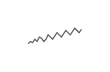
\begin{tikzpicture}[x=0.08em, y=0.08em, line width=0.4pt]
                \draw[FooterGray] (0,3) -- (1,4) -- (2,3.5) -- (3,5) -- (4,4) -- (5,6) -- (6,5.5) -- (7,4) -- (8,5) -- (9,7) -- (10,6) -- (11,5) -- (12,6.5) -- (13,8) -- (14,7) -- (15,6) -- (16,7.5) -- (17,9) -- (18,8) -- (19,7) -- (20,8.5) -- (21,10) -- (22,9) -- (23,8) -- (24,9.5);
            \end{tikzpicture}%
        }%
        \hskip0.5cm%
    }%
    \vskip6pt%
}

%=============================================================================
% PACKAGES
%=============================================================================
\usepackage[utf8]{inputenc}
\DeclareUnicodeCharacter{03B1}{\ensuremath{\alpha}}
\usepackage[T1]{fontenc}
\usepackage{amsmath, amssymb, amsthm}
\usepackage{mathtools}
\usepackage{bm}
\usepackage{tikz}
\usetikzlibrary{arrows.meta, positioning, shapes, calc, decorations.pathreplacing, shadings}
\usepackage{booktabs}
\usepackage{multirow}
\usepackage{array}
\usepackage{graphicx}
\usepackage{animate}
\usepackage{hyperref}
\usepackage{colortbl}
\usepackage{listings}
\lstset{language=Python, basicstyle=\ttfamily\scriptsize, keywordstyle=\color{MainBlue}\bfseries,
  commentstyle=\color{Forest}, stringstyle=\color{Crimson}, breaklines=true,
  frame=none, backgroundcolor=\color{VeryLightGray}, xleftmargin=2mm}
\hypersetup{colorlinks=true, linkcolor=MainBlue, urlcolor=MainBlue}
\graphicspath{{../../logos/}{../../charts/}{../../photos/}}
\usepackage{xcolor}
\hfuzz=2pt  % Suppress tiny overfull warnings (<2pt)
\vfuzz=2pt  % Suppress tiny vertical overfull warnings (<2pt)
% \mathrm in the sans-serif family of the slides (beamer resets \mathrm to the serif family at \begin{document};
% this hook runs after beamer's, so WN, Var, RMSE, ... in formulas match the surrounding text)
% Bold vectors and matrices in the same sans-serif family: \mathbf{A} in sans bold (beamer's own \mathbf came out in
% medium weight), and the bold upright Greek capitals of \boldsymbol / \bm (\bSigma, \bPhi, \boldsymbol{\Theta}) in
% cmss bold: bm.sty fixes its "boldoperators" font when it is loaded (serif cmbx), before beamer switches the
% operators to cmss, so it is reset here.
\AtBeginDocument{%
  \SetMathAlphabet{\mathrm}{normal}{\encodingdefault}{\sfdefault}{\mddefault}{n}%
  \SetMathAlphabet{\mathrm}{bold}{\encodingdefault}{\sfdefault}{bx}{n}%
  \SetMathAlphabet{\mathbf}{normal}{\encodingdefault}{\sfdefault}{bx}{n}%
  \SetMathAlphabet{\mathbf}{bold}{\encodingdefault}{\sfdefault}{bx}{n}%
  \SetSymbolFont{boldoperators}{normal}{OT1}{cmss}{bx}{n}%
  \SetSymbolFont{boldoperators}{bold}{OT1}{cmss}{bx}{n}}

%=============================================================================
% QUANTLET COMMANDS
%   \quantlet{<displayed name>}{<url>}       (generic, compatible with the older TSA decks)
%   \tsaquantlet{Ch_05}{TSA_ch5_garch}       -> https://github.com/danpele/Time-Series-Analysis/tree/main/Quantlets/Ch_05/TSA_ch5_garch
%   \qlurl{<folder>} is defined per chapter by the generator (Quantlets/Ch_NN/<folder>)
%=============================================================================
\newcommand{\tsarepo}{https://github.com/danpele/Time-Series-Analysis}
\newcommand{\tsaqlbase}{https://github.com/danpele/Time-Series-Analysis/tree/main/Quantlets}
\newcommand{\quantlet}[2]{%
    \hfill\href{#2}{%
        \raisebox{-0.15em}{
\includegraphics[height=0.7em]{ql_logo.png}}%
        \textcolor{MainBlue}{\tiny\ #1}%
    }%
}
\newcommand{\tsaquantlet}[2]{\quantlet{\detokenize{#2}}{\tsaqlbase/#1/#2}}

%=============================================================================
% NOTEBOOKS (Google Colab)
%   \colaburl{notebooks/EN/chapter5_seminar_notebook.ipynb} -> the Colab link of a file in the TSA repo
%   \nb: the chapter notebook (each seminar deck redefines it with \renewcommand)
%=============================================================================
\newcommand{\colaburl}[1]{https://colab.research.google.com/github/danpele/Time-Series-Analysis/blob/main/#1}
\newcommand{\nb}{https://colab.research.google.com/github/danpele/Time-Series-Analysis/tree/main/notebooks/EN}
\newcommand{\nbname}{notebooks/EN}

%=============================================================================
% SLIDE HELPERS (used by the generators; the same as in MFM)
%=============================================================================
% local font size for list bodies (the preamble forces \normalsize)
\newcommand{\itemsize}[1]{\setbeamertemplate{itemize/enumerate body begin}{#1}\setbeamertemplate{itemize/enumerate subbody begin}{#1}}
\newcommand{\intitle}[1]{{\hypersetup{urlcolor=white}#1}}   % white links inside coloured title bars
\newcommand{\imgcap}[1]{{\scriptsize #1}\\[0.5mm]}          % caption under a photo
\newcommand{\imgcredit}[2]{{\tiny\color{FooterGray}\href{#1}{#2}}}   % image credit: source URL, author/licence
\newcommand{\aiprompt}[1]{{\ttfamily\color{MainBlue}#1}}     % a prompt to an AI assistant

%=============================================================================
% SEMINARS: student version by default; the instructor wrapper *_solutions.tex sets \solutionstrue
%=============================================================================
\makeatletter\@ifundefined{ifsolutions}{\expandafter\newif\csname ifsolutions\endcsname}{}\makeatother
\newcommand{\solonly}[1]{\ifsolutions #1\fi}
\newcommand{\propsub}{\ifsolutions\else\framesubtitle{\ifdefined\tsalang Rezolvarea se discută la seminar\else Solution discussed in class\fi}\fi}

%=============================================================================
% APPENDIX AND CHAPTER LINKS (latex/appendix_links.py writes the calls; it also re-declares these
% macros before \begin{document}, so the decks compile with or without this preamble block)
%=============================================================================
\providecommand{\tsaapplink}[3]{\hypertarget{#2}{}\hyperlink{#1}{\beamergotobutton{#3}}}
\providecommand{\tsaappback}[2]{\begin{tikzpicture}[remember picture,overlay]\node[anchor=south east] at ([xshift=-3mm,yshift=7mm]current page.south east){\hyperlink{#1}{\beamerreturnbutton{#2}}};\end{tikzpicture}}
\providecommand{\tsachlink}[2]{\href{#1}{#2}}
\providecommand{\tsachlinkt}[2]{\href{#1}{\usebeamercolor[fg]{frametitle}#2}}

%=============================================================================
% QUANTINAR COMMAND: link către un curs Quantinar (subiecte avansate)
%=============================================================================
\newcommand{\quantinar}[2]{%
    \href{#2}{%
        \raisebox{-0.15em}{
\includegraphics[height=0.8em]{qr_logo.png}}%
        \textcolor{MainBlue}{\scriptsize\ #1}%
    }%
}

%=============================================================================
% CUSTOM TITLE PAGE
%=============================================================================
\defbeamertemplate*{title page}{hybrid}[1][]
{
    \vspace{0.2cm}
    % Logos row - top header (with clickable links)
    \begin{center}
        \href{https://www.ase.ro}{
\includegraphics[height=1.0cm]{ase_logo.png}}\hspace{0.3cm}%
        \href{https://theida.net}{
\includegraphics[height=1.0cm]{ida_logo.png}}\hspace{0.3cm}%
        \href{https://blockchain-research-center.com}{
\includegraphics[height=1.0cm]{brc_logo.png}}\hspace{0.3cm}%
        \href{https://www.ai4efin.ase.ro}{
\includegraphics[height=1.0cm]{ai4efin_logo.png}}\hspace{0.3cm}%
        \href{https://ipe.ro/new}{
\includegraphics[height=1.0cm]{acad_logo.png}}\hspace{0.3cm}%
        \href{https://www.digital-finance-msca.com}{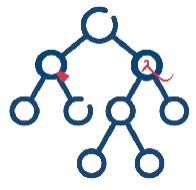
\includegraphics[height=1.0cm]{msca_logo.png}}%
    \end{center}

    \vspace{0.6cm}

    % Main title with Q logos on sides (with clickable links)
    \begin{center}
        \begin{minipage}{0.1\textwidth}
            \centering
            \href{https://quantlet.com}{
\includegraphics[height=1.1cm]{ql_logo.png}}
        \end{minipage}%
        \begin{minipage}{0.78\textwidth}
            \centering
            {\LARGE\bfseries\usebeamercolor[fg]{title}\inserttitle}

            \vspace{0.3cm}

            {\usebeamerfont{subtitle}\usebeamercolor[fg]{title}\insertsubtitle}
        \end{minipage}%
        \begin{minipage}{0.1\textwidth}
            \centering
            \href{https://quantinar.com}{
\includegraphics[height=1.1cm]{qr_logo.png}}
        \end{minipage}
    \end{center}

    \vspace{0.6cm}

    % Authors (left aligned)
    \hspace{0.5cm}{\usebeamerfont{author}\insertauthor}

    \vspace{0.3cm}

    % Institute/Affiliations (left aligned)
    \hspace{0.5cm}\begin{minipage}[t]{0.9\textwidth}
        \raggedright\small\insertinstitute
    \end{minipage}
}

%=============================================================================
% THEOREM ENVIRONMENTS
%=============================================================================
\theoremstyle{definition}
\setbeamertemplate{theorems}[numbered]
\ifdefined\tsalang
\newtheorem{defn}{Definiție}
\newtheorem{thm}{Teoremă}
\newtheorem{prop}{Propoziție}
\newtheorem{rmk}{Observație}
\else
\newtheorem{defn}{Definition}
\newtheorem{thm}{Theorem}
\newtheorem{prop}{Proposition}
\newtheorem{rmk}{Remark}
\fi

%=============================================================================
% CENTRED MINIPAGE (no extra vertical space)
%=============================================================================
\newenvironment{cminipage}[1]{%
    \par\noindent\hfill\begin{minipage}{#1}\ignorespaces
}{%
    \end{minipage}\hfill\null\par
}

%=============================================================================
% CUSTOM COMMANDS
%=============================================================================
\newcommand{\E}{\mathbb{E}}
\newcommand{\Var}{\text{Var}}
\newcommand{\Cov}{\text{Cov}}
\newcommand{\Corr}{\text{Corr}}
\newcommand{\R}{\mathbb{R}}
\newcommand{\N}{\mathbb{N}}
\newcommand{\Z}{\mathbb{Z}}
\newcommand{\B}{\mathbf{B}}
\newcommand{\imark}{\textcolor{MainBlue}{\textbullet}}
\newcommand{\RMSE}{\text{RMSE}}
\newcommand{\MAE}{\text{MAE}}
\newcommand{\MAPE}{\text{MAPE}}

% Boldface vector/matrix commands (VAR, VECM, state space; also used by the older TSA decks)
\newcommand{\bY}{\mathbf{Y}}
\newcommand{\bX}{\mathbf{X}}
\newcommand{\bA}{\mathbf{A}}
\newcommand{\bB}{\mathbf{B}}
\newcommand{\bepsilon}{\boldsymbol{\varepsilon}}
\newcommand{\bSigma}{\boldsymbol{\Sigma}}
\newcommand{\bPhi}{\boldsymbol{\Phi}}
\newcommand{\bGamma}{\boldsymbol{\Gamma}}
\newcommand{\bPi}{\boldsymbol{\Pi}}
\newcommand{\bc}{\mathbf{c}}
\newcommand{\balpha}{\boldsymbol{\alpha}}
\newcommand{\bbeta}{\boldsymbol{\beta}}
\newcommand{\bvarepsilon}{\boldsymbol{\varepsilon}}

% Legacy seminar marks (older TSA seminar decks)
\newcommand{\correct}{\textcolor{Forest}{\checkmark}}
\newcommand{\incorrect}{\textcolor{Crimson}{\texttimes}}
 se definește
%   \newcommand{\coursename}{Time Series Analysis}      (EN)
%   \newcommand{\coursename}{Serii de timp}       (RO)  și  \def\tsalang{ro}
% Fișierele .tex se află în EN/Courses, EN/Seminars, RO/Cursuri, RO/Seminarii (două niveluri sub rădăcină).
% Deck-urile sînt generate de latex/build_chapterN.py / build_seminarN.py (vezi latex/tsa_build.py).

\documentclass[9pt, aspectratio=169, t]{beamer}
\providecommand{\coursename}{Time Series Analysis}

% Ensure content fits on slides
\setbeamersize{text margin left=8mm, text margin right=8mm}
% Smaller institute font (title page)
\setbeamerfont{institute}{size=\footnotesize}

%=============================================================================
% THEME AND STYLE CONFIGURATION
%=============================================================================
\usetheme{default}
% Using default theme for clean header/footer control

% Color Palette (matching Redispatch PDF)
\definecolor{MainBlue}{RGB}{26, 58, 110}
\definecolor{AccentBlue}{RGB}{26, 58, 110}
\definecolor{IDAred}{RGB}{205, 0, 0}
\definecolor{DarkGray}{RGB}{51, 51, 51}
\definecolor{MediumGray}{RGB}{128, 128, 128}
\definecolor{LightGray}{RGB}{248, 248, 248}
\definecolor{VeryLightGray}{RGB}{235, 235, 235}
\definecolor{KeynoteGray}{RGB}{218, 218, 218}
\definecolor{SectionGray}{RGB}{120, 120, 120}
\definecolor{FooterGray}{RGB}{100, 100, 100}
\definecolor{Crimson}{RGB}{220, 53, 69}
\definecolor{Forest}{RGB}{46, 125, 50}
\definecolor{Amber}{RGB}{181, 133, 63}
\definecolor{Orange}{RGB}{230, 126, 34}
\definecolor{Purple}{RGB}{142, 68, 173}

% Gradient background (exact Keynote 315° gradient: white to RGB 218,218,218)
\setbeamertemplate{background}{%
    \begin{tikzpicture}[remember picture, overlay]
        \shade[shading=axis, shading angle=315,
        top color=white, bottom color=KeynoteGray]
        (current page.south west) rectangle (current page.north east);
    \end{tikzpicture}%
}
% Fallback solid color for compatibility
\setbeamercolor{background canvas}{bg=}

\setbeamercolor{palette primary}{bg=MainBlue, fg=white}
\setbeamercolor{palette secondary}{bg=MainBlue!85, fg=white}
\setbeamercolor{palette tertiary}{bg=MainBlue!70, fg=white}
\setbeamercolor{structure}{fg=MainBlue}
\setbeamercolor{title}{fg=IDAred}
\setbeamercolor{frametitle}{fg=IDAred, bg=}
\setbeamercolor{block title}{bg=MainBlue, fg=white}
\setbeamercolor{block body}{bg=VeryLightGray, fg=DarkGray}
\setbeamercolor{block title alerted}{bg=Crimson, fg=white}
\setbeamercolor{block body alerted}{bg=Crimson!8, fg=DarkGray}
\setbeamercolor{block title example}{bg=Forest, fg=white}
\setbeamercolor{block body example}{bg=Forest!8, fg=DarkGray}
\setbeamercolor{item}{fg=MainBlue}

% Footer colors (override Madrid theme blue)
\setbeamercolor{author in head/foot}{fg=FooterGray, bg=}
\setbeamercolor{title in head/foot}{fg=FooterGray, bg=}
\setbeamercolor{date in head/foot}{fg=FooterGray, bg=}
\setbeamercolor{section in head/foot}{fg=FooterGray, bg=}
\setbeamercolor{subsection in head/foot}{fg=FooterGray, bg=}

% Bullet styles (apply everywhere including blocks)
\setbeamertemplate{itemize item}{\color{MainBlue}$\boxdot$}
\setbeamertemplate{itemize subitem}{\color{MainBlue}$\blacktriangleright$}
\setbeamertemplate{itemize subsubitem}{\color{MainBlue}\tiny$\bullet$}
\setbeamertemplate{itemize/enumerate body begin}{\normalsize}
\setbeamertemplate{itemize/enumerate subbody begin}{\normalsize}

% Item spacing - compact style
\setlength{\leftmargini}{10pt}       % Level 1: minimal indent
\setlength{\leftmarginii}{10pt}      % Level 2: minimal additional indent
% Compact list spacing (zero extra space before/after lists in blocks)
\makeatletter
\def\@listi{\leftmargin\leftmargini \topsep 0pt \parsep 0pt \itemsep 0pt}
\def\@listii{\leftmargin\leftmarginii \topsep 0pt \parsep 0pt \itemsep 0pt}
\makeatother

\setbeamertemplate{navigation symbols}{}

%=============================================================================
% CUSTOM HEADLINE
%=============================================================================
\setbeamertemplate{headline}{%
    \vskip10pt%
    \hbox to \paperwidth{%
        \hskip0.5cm%
        {\small\color{FooterGray}\renewcommand{\hyperlink}[2]{##2}\insertsectionhead}%
        \hfill%
        \textcolor{FooterGray}{\small\insertframenumber}%
        \hskip0.5cm%
    }%
    \vskip4pt%
    {\color{FooterGray}\hrule height 0.4pt}%
}

%=============================================================================
% CUSTOM FOOTER
%=============================================================================
\usepackage{fontawesome5}

\setbeamertemplate{footline}{%
    {\color{FooterGray}\hrule height 0.4pt}%
    \vskip4pt%
    \hbox to \paperwidth{%
        \hskip0.5cm%
        \textcolor{FooterGray}{\small\coursename}%
        \hfill%
        \raisebox{-0.1em}{%
            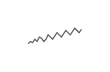
\begin{tikzpicture}[x=0.08em, y=0.08em, line width=0.4pt]
                \draw[FooterGray] (0,3) -- (1,4) -- (2,3.5) -- (3,5) -- (4,4) -- (5,6) -- (6,5.5) -- (7,4) -- (8,5) -- (9,7) -- (10,6) -- (11,5) -- (12,6.5) -- (13,8) -- (14,7) -- (15,6) -- (16,7.5) -- (17,9) -- (18,8) -- (19,7) -- (20,8.5) -- (21,10) -- (22,9) -- (23,8) -- (24,9.5);
            \end{tikzpicture}%
        }%
        \hskip0.5cm%
    }%
    \vskip6pt%
}

%=============================================================================
% PACKAGES
%=============================================================================
\usepackage[utf8]{inputenc}
\DeclareUnicodeCharacter{03B1}{\ensuremath{\alpha}}
\usepackage[T1]{fontenc}
\usepackage{amsmath, amssymb, amsthm}
\usepackage{mathtools}
\usepackage{bm}
\usepackage{tikz}
\usetikzlibrary{arrows.meta, positioning, shapes, calc, decorations.pathreplacing, shadings}
\usepackage{booktabs}
\usepackage{multirow}
\usepackage{array}
\usepackage{graphicx}
\usepackage{animate}
\usepackage{hyperref}
\usepackage{colortbl}
\usepackage{listings}
\lstset{language=Python, basicstyle=\ttfamily\scriptsize, keywordstyle=\color{MainBlue}\bfseries,
  commentstyle=\color{Forest}, stringstyle=\color{Crimson}, breaklines=true,
  frame=none, backgroundcolor=\color{VeryLightGray}, xleftmargin=2mm}
\hypersetup{colorlinks=true, linkcolor=MainBlue, urlcolor=MainBlue}
\graphicspath{{../../logos/}{../../charts/}{../../photos/}}
\usepackage{xcolor}
\hfuzz=2pt  % Suppress tiny overfull warnings (<2pt)
\vfuzz=2pt  % Suppress tiny vertical overfull warnings (<2pt)
% \mathrm in the sans-serif family of the slides (beamer resets \mathrm to the serif family at \begin{document};
% this hook runs after beamer's, so WN, Var, RMSE, ... in formulas match the surrounding text)
% Bold vectors and matrices in the same sans-serif family: \mathbf{A} in sans bold (beamer's own \mathbf came out in
% medium weight), and the bold upright Greek capitals of \boldsymbol / \bm (\bSigma, \bPhi, \boldsymbol{\Theta}) in
% cmss bold: bm.sty fixes its "boldoperators" font when it is loaded (serif cmbx), before beamer switches the
% operators to cmss, so it is reset here.
\AtBeginDocument{%
  \SetMathAlphabet{\mathrm}{normal}{\encodingdefault}{\sfdefault}{\mddefault}{n}%
  \SetMathAlphabet{\mathrm}{bold}{\encodingdefault}{\sfdefault}{bx}{n}%
  \SetMathAlphabet{\mathbf}{normal}{\encodingdefault}{\sfdefault}{bx}{n}%
  \SetMathAlphabet{\mathbf}{bold}{\encodingdefault}{\sfdefault}{bx}{n}%
  \SetSymbolFont{boldoperators}{normal}{OT1}{cmss}{bx}{n}%
  \SetSymbolFont{boldoperators}{bold}{OT1}{cmss}{bx}{n}}

%=============================================================================
% QUANTLET COMMANDS
%   \quantlet{<displayed name>}{<url>}       (generic, compatible with the older TSA decks)
%   \tsaquantlet{Ch_05}{TSA_ch5_garch}       -> https://github.com/danpele/Time-Series-Analysis/tree/main/Quantlets/Ch_05/TSA_ch5_garch
%   \qlurl{<folder>} is defined per chapter by the generator (Quantlets/Ch_NN/<folder>)
%=============================================================================
\newcommand{\tsarepo}{https://github.com/danpele/Time-Series-Analysis}
\newcommand{\tsaqlbase}{https://github.com/danpele/Time-Series-Analysis/tree/main/Quantlets}
\newcommand{\quantlet}[2]{%
    \hfill\href{#2}{%
        \raisebox{-0.15em}{
\includegraphics[height=0.7em]{ql_logo.png}}%
        \textcolor{MainBlue}{\tiny\ #1}%
    }%
}
\newcommand{\tsaquantlet}[2]{\quantlet{\detokenize{#2}}{\tsaqlbase/#1/#2}}

%=============================================================================
% NOTEBOOKS (Google Colab)
%   \colaburl{notebooks/EN/chapter5_seminar_notebook.ipynb} -> the Colab link of a file in the TSA repo
%   \nb: the chapter notebook (each seminar deck redefines it with \renewcommand)
%=============================================================================
\newcommand{\colaburl}[1]{https://colab.research.google.com/github/danpele/Time-Series-Analysis/blob/main/#1}
\newcommand{\nb}{https://colab.research.google.com/github/danpele/Time-Series-Analysis/tree/main/notebooks/EN}
\newcommand{\nbname}{notebooks/EN}

%=============================================================================
% SLIDE HELPERS (used by the generators; the same as in MFM)
%=============================================================================
% local font size for list bodies (the preamble forces \normalsize)
\newcommand{\itemsize}[1]{\setbeamertemplate{itemize/enumerate body begin}{#1}\setbeamertemplate{itemize/enumerate subbody begin}{#1}}
\newcommand{\intitle}[1]{{\hypersetup{urlcolor=white}#1}}   % white links inside coloured title bars
\newcommand{\imgcap}[1]{{\scriptsize #1}\\[0.5mm]}          % caption under a photo
\newcommand{\imgcredit}[2]{{\tiny\color{FooterGray}\href{#1}{#2}}}   % image credit: source URL, author/licence
\newcommand{\aiprompt}[1]{{\ttfamily\color{MainBlue}#1}}     % a prompt to an AI assistant

%=============================================================================
% SEMINARS: student version by default; the instructor wrapper *_solutions.tex sets \solutionstrue
%=============================================================================
\makeatletter\@ifundefined{ifsolutions}{\expandafter\newif\csname ifsolutions\endcsname}{}\makeatother
\newcommand{\solonly}[1]{\ifsolutions #1\fi}
\newcommand{\propsub}{\ifsolutions\else\framesubtitle{\ifdefined\tsalang Rezolvarea se discută la seminar\else Solution discussed in class\fi}\fi}

%=============================================================================
% APPENDIX AND CHAPTER LINKS (latex/appendix_links.py writes the calls; it also re-declares these
% macros before \begin{document}, so the decks compile with or without this preamble block)
%=============================================================================
\providecommand{\tsaapplink}[3]{\hypertarget{#2}{}\hyperlink{#1}{\beamergotobutton{#3}}}
\providecommand{\tsaappback}[2]{\begin{tikzpicture}[remember picture,overlay]\node[anchor=south east] at ([xshift=-3mm,yshift=7mm]current page.south east){\hyperlink{#1}{\beamerreturnbutton{#2}}};\end{tikzpicture}}
\providecommand{\tsachlink}[2]{\href{#1}{#2}}
\providecommand{\tsachlinkt}[2]{\href{#1}{\usebeamercolor[fg]{frametitle}#2}}

%=============================================================================
% QUANTINAR COMMAND: link către un curs Quantinar (subiecte avansate)
%=============================================================================
\newcommand{\quantinar}[2]{%
    \href{#2}{%
        \raisebox{-0.15em}{
\includegraphics[height=0.8em]{qr_logo.png}}%
        \textcolor{MainBlue}{\scriptsize\ #1}%
    }%
}

%=============================================================================
% CUSTOM TITLE PAGE
%=============================================================================
\defbeamertemplate*{title page}{hybrid}[1][]
{
    \vspace{0.2cm}
    % Logos row - top header (with clickable links)
    \begin{center}
        \href{https://www.ase.ro}{
\includegraphics[height=1.0cm]{ase_logo.png}}\hspace{0.3cm}%
        \href{https://theida.net}{
\includegraphics[height=1.0cm]{ida_logo.png}}\hspace{0.3cm}%
        \href{https://blockchain-research-center.com}{
\includegraphics[height=1.0cm]{brc_logo.png}}\hspace{0.3cm}%
        \href{https://www.ai4efin.ase.ro}{
\includegraphics[height=1.0cm]{ai4efin_logo.png}}\hspace{0.3cm}%
        \href{https://ipe.ro/new}{
\includegraphics[height=1.0cm]{acad_logo.png}}\hspace{0.3cm}%
        \href{https://www.digital-finance-msca.com}{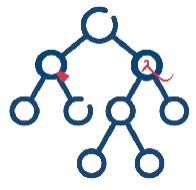
\includegraphics[height=1.0cm]{msca_logo.png}}%
    \end{center}

    \vspace{0.6cm}

    % Main title with Q logos on sides (with clickable links)
    \begin{center}
        \begin{minipage}{0.1\textwidth}
            \centering
            \href{https://quantlet.com}{
\includegraphics[height=1.1cm]{ql_logo.png}}
        \end{minipage}%
        \begin{minipage}{0.78\textwidth}
            \centering
            {\LARGE\bfseries\usebeamercolor[fg]{title}\inserttitle}

            \vspace{0.3cm}

            {\usebeamerfont{subtitle}\usebeamercolor[fg]{title}\insertsubtitle}
        \end{minipage}%
        \begin{minipage}{0.1\textwidth}
            \centering
            \href{https://quantinar.com}{
\includegraphics[height=1.1cm]{qr_logo.png}}
        \end{minipage}
    \end{center}

    \vspace{0.6cm}

    % Authors (left aligned)
    \hspace{0.5cm}{\usebeamerfont{author}\insertauthor}

    \vspace{0.3cm}

    % Institute/Affiliations (left aligned)
    \hspace{0.5cm}\begin{minipage}[t]{0.9\textwidth}
        \raggedright\small\insertinstitute
    \end{minipage}
}

%=============================================================================
% THEOREM ENVIRONMENTS
%=============================================================================
\theoremstyle{definition}
\setbeamertemplate{theorems}[numbered]
\ifdefined\tsalang
\newtheorem{defn}{Definiție}
\newtheorem{thm}{Teoremă}
\newtheorem{prop}{Propoziție}
\newtheorem{rmk}{Observație}
\else
\newtheorem{defn}{Definition}
\newtheorem{thm}{Theorem}
\newtheorem{prop}{Proposition}
\newtheorem{rmk}{Remark}
\fi

%=============================================================================
% CENTRED MINIPAGE (no extra vertical space)
%=============================================================================
\newenvironment{cminipage}[1]{%
    \par\noindent\hfill\begin{minipage}{#1}\ignorespaces
}{%
    \end{minipage}\hfill\null\par
}

%=============================================================================
% CUSTOM COMMANDS
%=============================================================================
\newcommand{\E}{\mathbb{E}}
\newcommand{\Var}{\text{Var}}
\newcommand{\Cov}{\text{Cov}}
\newcommand{\Corr}{\text{Corr}}
\newcommand{\R}{\mathbb{R}}
\newcommand{\N}{\mathbb{N}}
\newcommand{\Z}{\mathbb{Z}}
\newcommand{\B}{\mathbf{B}}
\newcommand{\imark}{\textcolor{MainBlue}{\textbullet}}
\newcommand{\RMSE}{\text{RMSE}}
\newcommand{\MAE}{\text{MAE}}
\newcommand{\MAPE}{\text{MAPE}}

% Boldface vector/matrix commands (VAR, VECM, state space; also used by the older TSA decks)
\newcommand{\bY}{\mathbf{Y}}
\newcommand{\bX}{\mathbf{X}}
\newcommand{\bA}{\mathbf{A}}
\newcommand{\bB}{\mathbf{B}}
\newcommand{\bepsilon}{\boldsymbol{\varepsilon}}
\newcommand{\bSigma}{\boldsymbol{\Sigma}}
\newcommand{\bPhi}{\boldsymbol{\Phi}}
\newcommand{\bGamma}{\boldsymbol{\Gamma}}
\newcommand{\bPi}{\boldsymbol{\Pi}}
\newcommand{\bc}{\mathbf{c}}
\newcommand{\balpha}{\boldsymbol{\alpha}}
\newcommand{\bbeta}{\boldsymbol{\beta}}
\newcommand{\bvarepsilon}{\boldsymbol{\varepsilon}}

% Legacy seminar marks (older TSA seminar decks)
\newcommand{\correct}{\textcolor{Forest}{\checkmark}}
\newcommand{\incorrect}{\textcolor{Crimson}{\texttimes}}
 se definește
%   \newcommand{\coursename}{Time Series Analysis}      (EN)
%   \newcommand{\coursename}{Serii de timp}       (RO)  și  \def\tsalang{ro}
% Fișierele .tex se află în EN/Courses, EN/Seminars, RO/Cursuri, RO/Seminarii (două niveluri sub rădăcină).
% Deck-urile sînt generate de latex/build_chapterN.py / build_seminarN.py (vezi latex/tsa_build.py).

\documentclass[9pt, aspectratio=169, t]{beamer}
\providecommand{\coursename}{Time Series Analysis}

% Ensure content fits on slides
\setbeamersize{text margin left=8mm, text margin right=8mm}
% Smaller institute font (title page)
\setbeamerfont{institute}{size=\footnotesize}

%=============================================================================
% THEME AND STYLE CONFIGURATION
%=============================================================================
\usetheme{default}
% Using default theme for clean header/footer control

% Color Palette (matching Redispatch PDF)
\definecolor{MainBlue}{RGB}{26, 58, 110}
\definecolor{AccentBlue}{RGB}{26, 58, 110}
\definecolor{IDAred}{RGB}{205, 0, 0}
\definecolor{DarkGray}{RGB}{51, 51, 51}
\definecolor{MediumGray}{RGB}{128, 128, 128}
\definecolor{LightGray}{RGB}{248, 248, 248}
\definecolor{VeryLightGray}{RGB}{235, 235, 235}
\definecolor{KeynoteGray}{RGB}{218, 218, 218}
\definecolor{SectionGray}{RGB}{120, 120, 120}
\definecolor{FooterGray}{RGB}{100, 100, 100}
\definecolor{Crimson}{RGB}{220, 53, 69}
\definecolor{Forest}{RGB}{46, 125, 50}
\definecolor{Amber}{RGB}{181, 133, 63}
\definecolor{Orange}{RGB}{230, 126, 34}
\definecolor{Purple}{RGB}{142, 68, 173}

% Gradient background (exact Keynote 315° gradient: white to RGB 218,218,218)
\setbeamertemplate{background}{%
    \begin{tikzpicture}[remember picture, overlay]
        \shade[shading=axis, shading angle=315,
        top color=white, bottom color=KeynoteGray]
        (current page.south west) rectangle (current page.north east);
    \end{tikzpicture}%
}
% Fallback solid color for compatibility
\setbeamercolor{background canvas}{bg=}

\setbeamercolor{palette primary}{bg=MainBlue, fg=white}
\setbeamercolor{palette secondary}{bg=MainBlue!85, fg=white}
\setbeamercolor{palette tertiary}{bg=MainBlue!70, fg=white}
\setbeamercolor{structure}{fg=MainBlue}
\setbeamercolor{title}{fg=IDAred}
\setbeamercolor{frametitle}{fg=IDAred, bg=}
\setbeamercolor{block title}{bg=MainBlue, fg=white}
\setbeamercolor{block body}{bg=VeryLightGray, fg=DarkGray}
\setbeamercolor{block title alerted}{bg=Crimson, fg=white}
\setbeamercolor{block body alerted}{bg=Crimson!8, fg=DarkGray}
\setbeamercolor{block title example}{bg=Forest, fg=white}
\setbeamercolor{block body example}{bg=Forest!8, fg=DarkGray}
\setbeamercolor{item}{fg=MainBlue}

% Footer colors (override Madrid theme blue)
\setbeamercolor{author in head/foot}{fg=FooterGray, bg=}
\setbeamercolor{title in head/foot}{fg=FooterGray, bg=}
\setbeamercolor{date in head/foot}{fg=FooterGray, bg=}
\setbeamercolor{section in head/foot}{fg=FooterGray, bg=}
\setbeamercolor{subsection in head/foot}{fg=FooterGray, bg=}

% Bullet styles (apply everywhere including blocks)
\setbeamertemplate{itemize item}{\color{MainBlue}$\boxdot$}
\setbeamertemplate{itemize subitem}{\color{MainBlue}$\blacktriangleright$}
\setbeamertemplate{itemize subsubitem}{\color{MainBlue}\tiny$\bullet$}
\setbeamertemplate{itemize/enumerate body begin}{\normalsize}
\setbeamertemplate{itemize/enumerate subbody begin}{\normalsize}

% Item spacing - compact style
\setlength{\leftmargini}{10pt}       % Level 1: minimal indent
\setlength{\leftmarginii}{10pt}      % Level 2: minimal additional indent
% Compact list spacing (zero extra space before/after lists in blocks)
\makeatletter
\def\@listi{\leftmargin\leftmargini \topsep 0pt \parsep 0pt \itemsep 0pt}
\def\@listii{\leftmargin\leftmarginii \topsep 0pt \parsep 0pt \itemsep 0pt}
\makeatother

\setbeamertemplate{navigation symbols}{}

%=============================================================================
% CUSTOM HEADLINE
%=============================================================================
\setbeamertemplate{headline}{%
    \vskip10pt%
    \hbox to \paperwidth{%
        \hskip0.5cm%
        {\small\color{FooterGray}\renewcommand{\hyperlink}[2]{##2}\insertsectionhead}%
        \hfill%
        \textcolor{FooterGray}{\small\insertframenumber}%
        \hskip0.5cm%
    }%
    \vskip4pt%
    {\color{FooterGray}\hrule height 0.4pt}%
}

%=============================================================================
% CUSTOM FOOTER
%=============================================================================
\usepackage{fontawesome5}

\setbeamertemplate{footline}{%
    {\color{FooterGray}\hrule height 0.4pt}%
    \vskip4pt%
    \hbox to \paperwidth{%
        \hskip0.5cm%
        \textcolor{FooterGray}{\small\coursename}%
        \hfill%
        \raisebox{-0.1em}{%
            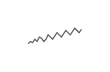
\begin{tikzpicture}[x=0.08em, y=0.08em, line width=0.4pt]
                \draw[FooterGray] (0,3) -- (1,4) -- (2,3.5) -- (3,5) -- (4,4) -- (5,6) -- (6,5.5) -- (7,4) -- (8,5) -- (9,7) -- (10,6) -- (11,5) -- (12,6.5) -- (13,8) -- (14,7) -- (15,6) -- (16,7.5) -- (17,9) -- (18,8) -- (19,7) -- (20,8.5) -- (21,10) -- (22,9) -- (23,8) -- (24,9.5);
            \end{tikzpicture}%
        }%
        \hskip0.5cm%
    }%
    \vskip6pt%
}

%=============================================================================
% PACKAGES
%=============================================================================
\usepackage[utf8]{inputenc}
\DeclareUnicodeCharacter{03B1}{\ensuremath{\alpha}}
\usepackage[T1]{fontenc}
\usepackage{amsmath, amssymb, amsthm}
\usepackage{mathtools}
\usepackage{bm}
\usepackage{tikz}
\usetikzlibrary{arrows.meta, positioning, shapes, calc, decorations.pathreplacing, shadings}
\usepackage{booktabs}
\usepackage{multirow}
\usepackage{array}
\usepackage{graphicx}
\usepackage{animate}
\usepackage{hyperref}
\usepackage{colortbl}
\usepackage{listings}
\lstset{language=Python, basicstyle=\ttfamily\scriptsize, keywordstyle=\color{MainBlue}\bfseries,
  commentstyle=\color{Forest}, stringstyle=\color{Crimson}, breaklines=true,
  frame=none, backgroundcolor=\color{VeryLightGray}, xleftmargin=2mm}
\hypersetup{colorlinks=true, linkcolor=MainBlue, urlcolor=MainBlue}
\graphicspath{{../../logos/}{../../charts/}{../../photos/}}
\usepackage{xcolor}
\hfuzz=2pt  % Suppress tiny overfull warnings (<2pt)
\vfuzz=2pt  % Suppress tiny vertical overfull warnings (<2pt)
% \mathrm in the sans-serif family of the slides (beamer resets \mathrm to the serif family at \begin{document};
% this hook runs after beamer's, so WN, Var, RMSE, ... in formulas match the surrounding text)
% Bold vectors and matrices in the same sans-serif family: \mathbf{A} in sans bold (beamer's own \mathbf came out in
% medium weight), and the bold upright Greek capitals of \boldsymbol / \bm (\bSigma, \bPhi, \boldsymbol{\Theta}) in
% cmss bold: bm.sty fixes its "boldoperators" font when it is loaded (serif cmbx), before beamer switches the
% operators to cmss, so it is reset here.
\AtBeginDocument{%
  \SetMathAlphabet{\mathrm}{normal}{\encodingdefault}{\sfdefault}{\mddefault}{n}%
  \SetMathAlphabet{\mathrm}{bold}{\encodingdefault}{\sfdefault}{bx}{n}%
  \SetMathAlphabet{\mathbf}{normal}{\encodingdefault}{\sfdefault}{bx}{n}%
  \SetMathAlphabet{\mathbf}{bold}{\encodingdefault}{\sfdefault}{bx}{n}%
  \SetSymbolFont{boldoperators}{normal}{OT1}{cmss}{bx}{n}%
  \SetSymbolFont{boldoperators}{bold}{OT1}{cmss}{bx}{n}}

%=============================================================================
% QUANTLET COMMANDS
%   \quantlet{<displayed name>}{<url>}       (generic, compatible with the older TSA decks)
%   \tsaquantlet{Ch_05}{TSA_ch5_garch}       -> https://github.com/danpele/Time-Series-Analysis/tree/main/Quantlets/Ch_05/TSA_ch5_garch
%   \qlurl{<folder>} is defined per chapter by the generator (Quantlets/Ch_NN/<folder>)
%=============================================================================
\newcommand{\tsarepo}{https://github.com/danpele/Time-Series-Analysis}
\newcommand{\tsaqlbase}{https://github.com/danpele/Time-Series-Analysis/tree/main/Quantlets}
\newcommand{\quantlet}[2]{%
    \hfill\href{#2}{%
        \raisebox{-0.15em}{
\includegraphics[height=0.7em]{ql_logo.png}}%
        \textcolor{MainBlue}{\tiny\ #1}%
    }%
}
\newcommand{\tsaquantlet}[2]{\quantlet{\detokenize{#2}}{\tsaqlbase/#1/#2}}

%=============================================================================
% NOTEBOOKS (Google Colab)
%   \colaburl{notebooks/EN/chapter5_seminar_notebook.ipynb} -> the Colab link of a file in the TSA repo
%   \nb: the chapter notebook (each seminar deck redefines it with \renewcommand)
%=============================================================================
\newcommand{\colaburl}[1]{https://colab.research.google.com/github/danpele/Time-Series-Analysis/blob/main/#1}
\newcommand{\nb}{https://colab.research.google.com/github/danpele/Time-Series-Analysis/tree/main/notebooks/EN}
\newcommand{\nbname}{notebooks/EN}

%=============================================================================
% SLIDE HELPERS (used by the generators; the same as in MFM)
%=============================================================================
% local font size for list bodies (the preamble forces \normalsize)
\newcommand{\itemsize}[1]{\setbeamertemplate{itemize/enumerate body begin}{#1}\setbeamertemplate{itemize/enumerate subbody begin}{#1}}
\newcommand{\intitle}[1]{{\hypersetup{urlcolor=white}#1}}   % white links inside coloured title bars
\newcommand{\imgcap}[1]{{\scriptsize #1}\\[0.5mm]}          % caption under a photo
\newcommand{\imgcredit}[2]{{\tiny\color{FooterGray}\href{#1}{#2}}}   % image credit: source URL, author/licence
\newcommand{\aiprompt}[1]{{\ttfamily\color{MainBlue}#1}}     % a prompt to an AI assistant

%=============================================================================
% SEMINARS: student version by default; the instructor wrapper *_solutions.tex sets \solutionstrue
%=============================================================================
\makeatletter\@ifundefined{ifsolutions}{\expandafter\newif\csname ifsolutions\endcsname}{}\makeatother
\newcommand{\solonly}[1]{\ifsolutions #1\fi}
\newcommand{\propsub}{\ifsolutions\else\framesubtitle{\ifdefined\tsalang Rezolvarea se discută la seminar\else Solution discussed in class\fi}\fi}

%=============================================================================
% APPENDIX AND CHAPTER LINKS (latex/appendix_links.py writes the calls; it also re-declares these
% macros before \begin{document}, so the decks compile with or without this preamble block)
%=============================================================================
\providecommand{\tsaapplink}[3]{\hypertarget{#2}{}\hyperlink{#1}{\beamergotobutton{#3}}}
\providecommand{\tsaappback}[2]{\begin{tikzpicture}[remember picture,overlay]\node[anchor=south east] at ([xshift=-3mm,yshift=7mm]current page.south east){\hyperlink{#1}{\beamerreturnbutton{#2}}};\end{tikzpicture}}
\providecommand{\tsachlink}[2]{\href{#1}{#2}}
\providecommand{\tsachlinkt}[2]{\href{#1}{\usebeamercolor[fg]{frametitle}#2}}

%=============================================================================
% QUANTINAR COMMAND: link către un curs Quantinar (subiecte avansate)
%=============================================================================
\newcommand{\quantinar}[2]{%
    \href{#2}{%
        \raisebox{-0.15em}{
\includegraphics[height=0.8em]{qr_logo.png}}%
        \textcolor{MainBlue}{\scriptsize\ #1}%
    }%
}

%=============================================================================
% CUSTOM TITLE PAGE
%=============================================================================
\defbeamertemplate*{title page}{hybrid}[1][]
{
    \vspace{0.2cm}
    % Logos row - top header (with clickable links)
    \begin{center}
        \href{https://www.ase.ro}{
\includegraphics[height=1.0cm]{ase_logo.png}}\hspace{0.3cm}%
        \href{https://theida.net}{
\includegraphics[height=1.0cm]{ida_logo.png}}\hspace{0.3cm}%
        \href{https://blockchain-research-center.com}{
\includegraphics[height=1.0cm]{brc_logo.png}}\hspace{0.3cm}%
        \href{https://www.ai4efin.ase.ro}{
\includegraphics[height=1.0cm]{ai4efin_logo.png}}\hspace{0.3cm}%
        \href{https://ipe.ro/new}{
\includegraphics[height=1.0cm]{acad_logo.png}}\hspace{0.3cm}%
        \href{https://www.digital-finance-msca.com}{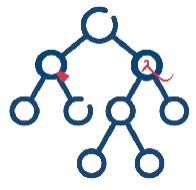
\includegraphics[height=1.0cm]{msca_logo.png}}%
    \end{center}

    \vspace{0.6cm}

    % Main title with Q logos on sides (with clickable links)
    \begin{center}
        \begin{minipage}{0.1\textwidth}
            \centering
            \href{https://quantlet.com}{
\includegraphics[height=1.1cm]{ql_logo.png}}
        \end{minipage}%
        \begin{minipage}{0.78\textwidth}
            \centering
            {\LARGE\bfseries\usebeamercolor[fg]{title}\inserttitle}

            \vspace{0.3cm}

            {\usebeamerfont{subtitle}\usebeamercolor[fg]{title}\insertsubtitle}
        \end{minipage}%
        \begin{minipage}{0.1\textwidth}
            \centering
            \href{https://quantinar.com}{
\includegraphics[height=1.1cm]{qr_logo.png}}
        \end{minipage}
    \end{center}

    \vspace{0.6cm}

    % Authors (left aligned)
    \hspace{0.5cm}{\usebeamerfont{author}\insertauthor}

    \vspace{0.3cm}

    % Institute/Affiliations (left aligned)
    \hspace{0.5cm}\begin{minipage}[t]{0.9\textwidth}
        \raggedright\small\insertinstitute
    \end{minipage}
}

%=============================================================================
% THEOREM ENVIRONMENTS
%=============================================================================
\theoremstyle{definition}
\setbeamertemplate{theorems}[numbered]
\ifdefined\tsalang
\newtheorem{defn}{Definiție}
\newtheorem{thm}{Teoremă}
\newtheorem{prop}{Propoziție}
\newtheorem{rmk}{Observație}
\else
\newtheorem{defn}{Definition}
\newtheorem{thm}{Theorem}
\newtheorem{prop}{Proposition}
\newtheorem{rmk}{Remark}
\fi

%=============================================================================
% CENTRED MINIPAGE (no extra vertical space)
%=============================================================================
\newenvironment{cminipage}[1]{%
    \par\noindent\hfill\begin{minipage}{#1}\ignorespaces
}{%
    \end{minipage}\hfill\null\par
}

%=============================================================================
% CUSTOM COMMANDS
%=============================================================================
\newcommand{\E}{\mathbb{E}}
\newcommand{\Var}{\text{Var}}
\newcommand{\Cov}{\text{Cov}}
\newcommand{\Corr}{\text{Corr}}
\newcommand{\R}{\mathbb{R}}
\newcommand{\N}{\mathbb{N}}
\newcommand{\Z}{\mathbb{Z}}
\newcommand{\B}{\mathbf{B}}
\newcommand{\imark}{\textcolor{MainBlue}{\textbullet}}
\newcommand{\RMSE}{\text{RMSE}}
\newcommand{\MAE}{\text{MAE}}
\newcommand{\MAPE}{\text{MAPE}}

% Boldface vector/matrix commands (VAR, VECM, state space; also used by the older TSA decks)
\newcommand{\bY}{\mathbf{Y}}
\newcommand{\bX}{\mathbf{X}}
\newcommand{\bA}{\mathbf{A}}
\newcommand{\bB}{\mathbf{B}}
\newcommand{\bepsilon}{\boldsymbol{\varepsilon}}
\newcommand{\bSigma}{\boldsymbol{\Sigma}}
\newcommand{\bPhi}{\boldsymbol{\Phi}}
\newcommand{\bGamma}{\boldsymbol{\Gamma}}
\newcommand{\bPi}{\boldsymbol{\Pi}}
\newcommand{\bc}{\mathbf{c}}
\newcommand{\balpha}{\boldsymbol{\alpha}}
\newcommand{\bbeta}{\boldsymbol{\beta}}
\newcommand{\bvarepsilon}{\boldsymbol{\varepsilon}}

% Legacy seminar marks (older TSA seminar decks)
\newcommand{\correct}{\textcolor{Forest}{\checkmark}}
\newcommand{\incorrect}{\textcolor{Crimson}{\texttimes}}


\newcommand{\qlurl}[1]{https://github.com/danpele/Time-Series-Analysis/tree/main/Quantlets/Ch_06/#1}

% Clickable citations (DOIs verified via Crossref)
\newcommand{\refHP}{\href{https://doi.org/10.1007/978-3-031-13584-2}{Huang and Petukhina (2022)}}
\newcommand{\refFPP}{\href{https://otexts.com/fpp3/VAR.html}{Hyndman and Athanasopoulos (2021)}}
\newcommand{\refLut}{\href{https://doi.org/10.1007/978-3-540-27752-1}{Lütkepohl (2005)}}
\newcommand{\refHamilton}{\href{https://doi.org/10.2307/j.ctv14jx6sm}{Hamilton (1994)}}
\newcommand{\refSims}{\href{https://doi.org/10.2307/1912017}{Sims (1980)}}
\newcommand{\refSimsPP}{\href{https://doi.org/10.1016/0014-2921(92)90041-T}{Sims (1992)}}
\newcommand{\refGranger}{\href{https://doi.org/10.2307/1912791}{Granger (1969)}}
\newcommand{\refLutOm}{\href{https://doi.org/10.1016/0304-4076(82)90011-2}{Lütkepohl (1982)}}
\newcommand{\refTY}{\href{https://doi.org/10.1016/0304-4076(94)01616-8}{Toda and Yamamoto (1995)}}
\newcommand{\refSSW}{\href{https://doi.org/10.2307/2938337}{Sims, Stock and Watson (1990)}}
\newcommand{\refSW}{\href{https://doi.org/10.1257/jep.15.4.101}{Stock and Watson (2001)}}
\newcommand{\refPS}{\href{https://doi.org/10.1016/S0165-1765(97)00214-0}{Pesaran and Shin (1998)}}
\newcommand{\refKPP}{\href{https://doi.org/10.1016/0304-4076(95)01753-4}{Koop, Pesaran and Potter (1996)}}
\newcommand{\refDY}{\href{https://doi.org/10.1111/j.1468-0297.2008.02208.x}{Diebold and Yilmaz (2009)}}
\newcommand{\refDYb}{\href{https://doi.org/10.1016/j.ijforecast.2011.02.006}{Diebold and Yilmaz (2012)}}
\newcommand{\refKilian}{\href{https://doi.org/10.1162/003465398557465}{Kilian (1998)}}
\newcommand{\refHosking}{\href{https://doi.org/10.1080/01621459.1980.10477520}{Hosking (1980)}}
\newcommand{\refJB}{\href{https://doi.org/10.1016/0165-1765(80)90024-5}{Jarque and Bera (1980)}}
\newcommand{\refAkaike}{\href{https://doi.org/10.1109/TAC.1974.1100705}{Akaike (1974)}}
\newcommand{\refSchwarz}{\href{https://doi.org/10.1214/aos/1176344136}{Schwarz (1978)}}
\newcommand{\refHQ}{\href{https://doi.org/10.1111/j.2517-6161.1979.tb01072.x}{Hannan and Quinn (1979)}}
\newcommand{\refDM}{\href{https://doi.org/10.1080/07350015.1995.10524599}{Diebold and Mariano (1995)}}
\newcommand{\refEG}{\href{https://doi.org/10.2307/1913236}{Engle and Granger (1987)}}

\title[Time Series Analysis]{Time Series Analysis}
\subtitle{Chapter 6: VAR models and Granger causality}
\author[D.T. Pele]{Daniel Traian PELE}
\institute{Bucharest University of Economic Studies\\
IDA Institute Digital Assets\\
Blockchain Research Center\\
AI4EFin Artificial Intelligence for Energy Finance\\
Romanian Academy, Institute for Economic Forecasting\\
MSCA Digital Finance}
\date{}

%=============================================================================
\providecommand{\tsaapplink}[3]{\hypertarget{#2}{}\hyperlink{#1}{\beamergotobutton{#3}}}  % APPLINKS-MACROS
\providecommand{\tsaappback}[2]{\begin{tikzpicture}[remember picture,overlay]\node[anchor=south east] at ([xshift=-3mm,yshift=7mm]current page.south east){\hyperlink{#1}{\beamerreturnbutton{#2}}};\end{tikzpicture}}  % APPLINKS-MACROS
\providecommand{\tsachlink}[2]{\href{#1}{#2}}  % APPLINKS-MACROS
\providecommand{\tsachlinkt}[2]{\href{#1}{\usebeamercolor[fg]{frametitle}#2}}  % APPLINKS-MACROS
\begin{document}
%=============================================================================

{
\setbeamertemplate{headline}{}
\setbeamertemplate{footline}{}
\begin{frame}[noframenumbering]
    \titlepage
\end{frame}
}
% BEGIN-ACRONYMS (generat de latex/acronyms.py; nu editati manual)
\begin{frame}{Acronyms used in this material}
\setbeamertemplate{itemize/enumerate body begin}{\footnotesize}
\begin{columns}[T]
\begin{column}{0.49\textwidth}
\begin{itemize}\setlength{\itemsep}{0pt}
    \item \textbf{AI}: Artificial Intelligence
    \item \textbf{AIC}: Akaike Information Criterion
    \item \textbf{AR}: AutoRegressive (model)
    \item \textbf{ARMA}: AutoRegressive Moving Average (model)
    \item \textbf{BET}: Bucharest Exchange Trading (index)
    \item \textbf{BIC}: Bayesian Information Criterion
    \item \textbf{BNR}: Banca Națională a României (the National Bank of Romania)
    \item \textbf{CCF}: Cross-Correlation Function
    \item \textbf{COVID-19}: COronaVIrus Disease 2019
    \item \textbf{DM}: Diebold–Mariano (test)
    \item \textbf{DSGE}: Dynamic Stochastic General Equilibrium (model)
    \item \textbf{EODHD}: EOD Historical Data (market-data provider)
    \item \textbf{EU}: European Union
    \item \textbf{FEVD}: Forecast Error Variance Decomposition
    \item \textbf{FRED}: Federal Reserve Economic Data
\end{itemize}
\end{column}
\begin{column}{0.49\textwidth}
\begin{itemize}\setlength{\itemsep}{0pt}
    \item \textbf{GDP}: Gross Domestic Product
    \item \textbf{GLS}: Generalised Least Squares
    \item \textbf{HICP}: Harmonised Index of Consumer Prices
    \item \textbf{HQ}: Hannan–Quinn (information criterion)
    \item \textbf{IRF}: Impulse Response Function
    \item \textbf{MA}: Moving Average
    \item \textbf{MSE}: Mean Squared Error
    \item \textbf{OLS}: Ordinary Least Squares
    \item \textbf{RMSE}: Root Mean Squared Error
    \item \textbf{ROBOR}: Romanian Interbank Offer Rate
    \item \textbf{RSS}: Residual Sum of Squares
    \item \textbf{SE}: Standard Error
    \item \textbf{SVAR}: Structural Vector AutoRegression
    \item \textbf{US}: United States
    \item \textbf{VAR}: Vector AutoRegression
    \item \textbf{VECM}: Vector Error Correction Model
\end{itemize}
\end{column}
\end{columns}
\end{frame}
% END-ACRONYMS

\begin{frame}{Today's question and route}
\itemsize{\small}
\begin{itemize}
    \item \textbf{Question}: when several series move together (output, prices, interest rates; three stock markets), how do we model them jointly, and what can we learn about who leads whom?
    \begin{itemize}
        \item one equation per variable, each with the past of all variables: the vector autoregression (VAR)
    \end{itemize}
    \item \textbf{Route} of the chapter
    \begin{itemize}
        \item from one series to several: vector processes and cross-correlations; the VAR$(p)$ model and its stability
        \item estimation, lag selection and diagnostics; Granger causality and its pitfalls
        \item impulse responses, variance decomposition, forecasts; the structural VAR idea of Sims (1980)
    \end{itemize}
    \item We build on \tsachlink{https://danpele.github.io/Time-Series-Analysis/EN/Courses/chapter2_arma_models.pdf}{Chapter 2} (AR models) and \tsachlink{https://danpele.github.io/Time-Series-Analysis/EN/Courses/chapter3_unit_roots_arima_models.pdf}{Chapter 3} (stationarity tests)
\end{itemize}
\end{frame}

\begin{frame}{Learning outcomes}
\itemsize{\small}
\begin{itemize}
    \item Write a VAR$(p)$ in matrix form and equation by equation, and count its parameters
    \item Check stability with the eigenvalues of the companion matrix, and compute the mean of a stable VAR
    \item Estimate a VAR by OLS, choose $p$ with AIC, BIC and HQ, and check the residuals
    \item Test Granger causality and explain what it does not prove
    \item Compute and read orthogonalised impulse responses and variance decompositions, and explain why the ordering matters
    \item Forecast with a VAR and compare it fairly with univariate benchmarks
\end{itemize}
\end{frame}

\begin{frame}{Reading and tools}
\itemsize{\small}
\begin{itemize}
    \item Textbook: \refHP, Ch.~7 (multivariate time series)
    \begin{itemize}
        \item companion, free online: \refFPP, Sec.~12.3 (vector autoregressions)
    \end{itemize}
    \item Theory: \refLut, Ch.~2--4; \refHamilton, Ch.~11; an accessible survey: \refSW
    \item Python Quantlets of this chapter: \href{https://github.com/danpele/Time-Series-Analysis/tree/main/Quantlets/Ch_06}{Quantlets/Ch\_06}
    \begin{itemize}
        \item \texttt{VAR} from \texttt{statsmodels}: \texttt{select\_order}, \texttt{fit}, \texttt{test\_whiteness}, \texttt{irf}, \texttt{fevd}, \texttt{forecast\_interval}
    \end{itemize}
    \item Lecture notebook: \href{\colaburl{notebooks/EN/chapter6_lecture_notebook.ipynb}}{open in Google Colab}
    \item Video course: \quantinar{Applied Time Series Analysis with Python}{https://quantinar.com/course/137/applied-time-series-analysis-with-python}
\end{itemize}
\end{frame}


%=============================================================================
\section{From one series to several}
%=============================================================================

\begin{frame}{Romania: four macro series that move together}
\itemsize{\footnotesize}
\begin{center}
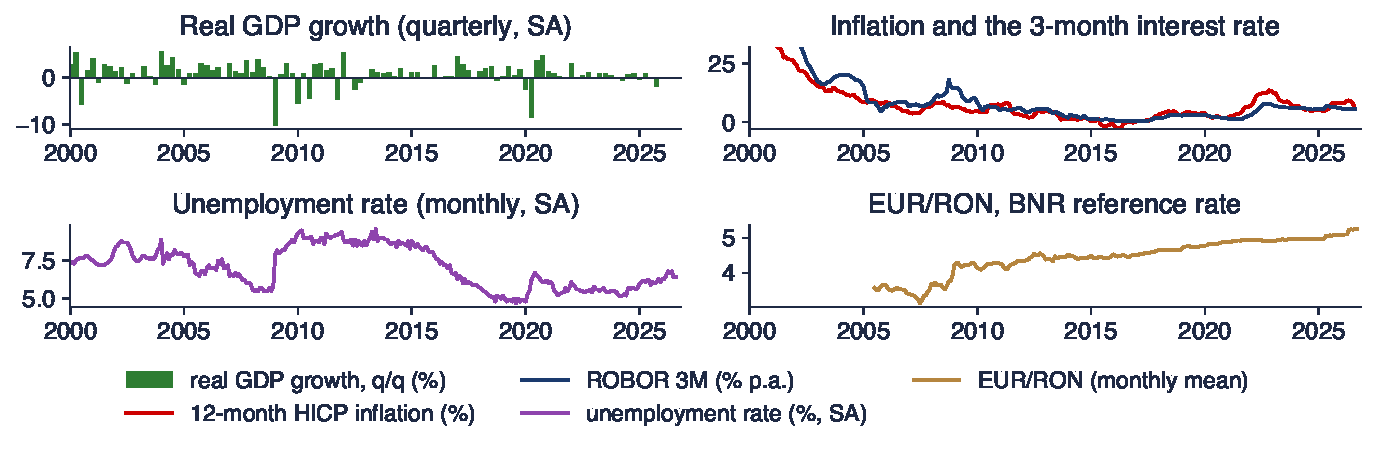
\includegraphics[width=0.97\textwidth,height=0.6\textheight,keepaspectratio]{tsa_ch6_ro_macro.pdf}
\end{center}
\vspace{-0.25cm}
\begin{itemize}
    \item Real GDP growth (q/q) and unemployment rate, seasonally adjusted; 12-month HICP inflation; ROBOR 3M, the 3-month interbank rate; source: Eurostat; EUR/RON: the BNR reference rate
\end{itemize}
\quantlet{TSA\_ch6\_multivariate\_data}{\qlurl{TSA_ch6_multivariate_data}}
\end{frame}

\begin{frame}{Interpreting the Romanian series}
\itemsize{\small}
\begin{itemize}
    \item Inflation and ROBOR 3M rise and fall together: correlation 0.66 over 2005Q1--2026Q2 (quarterly means)
    \begin{itemize}
        \item inflation peaked at 13.6\% in November 2022; ROBOR 3M peaked at 18.2\% in October 2008 (the 2008 liquidity squeeze)
    \end{itemize}
    \item GDP growth is noisy, with two deep falls: $-$10.2\% in 2009Q1 and $-$8.6\% in 2020Q2
    \begin{itemize}
        \item latest values: inflation 6.1\% (August 2026), ROBOR 3M 5.69\%, unemployment 6.4\%, EUR/RON 5.26
    \end{itemize}
    \item Questions for this chapter
    \begin{itemize}
        \item Does inflation help to forecast the interest rate?
        \item How does ROBOR react to an inflation surprise, and for how long?
    \end{itemize}
\end{itemize}
\end{frame}

\begin{frame}{Vector time series}
\itemsize{\small}
\begin{itemize}
    \item \textbf{Definition}: $\bY_t = (Y_{1t}, \dots, Y_{Kt})'$ collects $K$ series observed at the same dates
    \begin{itemize}
        \item example: $\bY_t = (g_t, \pi_t, i_t)'$, GDP growth, inflation and ROBOR 3M of quarter $t$; $K = 3$
        \item $Y_{jt}$: the value of series $j$ at date $t$; the prime $'$ denotes the transpose (a column vector)
    \end{itemize}
    \item \textbf{Mean vector}: $\boldsymbol{\mu} = E[\bY_t]$, $K \times 1$
    \begin{itemize}
        \item \textbf{autocovariance matrix} at lag $h$: $\bGamma(h) = \Cov(\bY_t, \bY_{t-h}) = E[(\bY_t - \boldsymbol{\mu})(\bY_{t-h} - \boldsymbol{\mu})']$, $K \times K$
        \item diagonal: the autocovariances of each series (\tsachlink{https://danpele.github.io/Time-Series-Analysis/EN/Courses/chapter1_stochastic_processes_stationarity.pdf}{Chapter 1}); off-diagonal: \textbf{cross-covariances} $\gamma_{jk}(h) = \Cov(Y_{jt}, Y_{k,t-h})$
    \end{itemize}
    \item \textbf{Weak stationarity}: $\boldsymbol{\mu}$ and $\bGamma(h)$ do not depend on $t$
    \begin{itemize}
        \item $\bGamma(h)$ is not symmetric, but $\bGamma(-h) = \bGamma(h)'$: ``$Y_1$ leads $Y_2$'' and ``$Y_2$ leads $Y_1$'' are different statements
    \end{itemize}
\end{itemize}
\end{frame}

\begin{frame}{The cross-correlation function}
\itemsize{\small}
\begin{itemize}
    \item \textbf{Definition}: $\rho_{yx}(k) = \Corr(y_t, x_{t-k}) = \gamma_{yx}(k)/(\sigma_y\sigma_x)$, for $k = 0, \pm 1, \pm 2, \dots$
    \begin{itemize}
        \item the cross-correlation function (CCF): $k > 0$: past $x$ with today's $y$ ($x$ leads); $k < 0$: $y$ leads
        \item $\gamma_{yx}(k) = \Cov(y_t, x_{t-k})$: the cross-covariance; $\sigma_y$, $\sigma_x$: the standard deviations of the two series
    \end{itemize}
    \item Sample version: $\hat\rho_{yx}(k)$, the correlation of the pairs $(y_t, x_{t-k})$
    \begin{itemize}
        \item if the two series are independent white noises, $\hat\rho_{yx}(k) \approx N(0, 1/T)$, with $T$ the number of observations: bands $\pm 1.96/\sqrt{T}$
        \item with autocorrelated series the bands are too narrow: spurious lead--lag patterns (compare \tsachlink{https://danpele.github.io/Time-Series-Analysis/EN/Courses/chapter3_unit_roots_arima_models.pdf}{Chapter 3}, spurious regression)
    \end{itemize}
    \item The CCF looks at one pair and one lag at a time; a VAR looks at all variables and all lags together
\end{itemize}
\end{frame}

\begin{frame}{Cross-correlations: markets and Romanian macro data}
\itemsize{\footnotesize}
\begin{center}
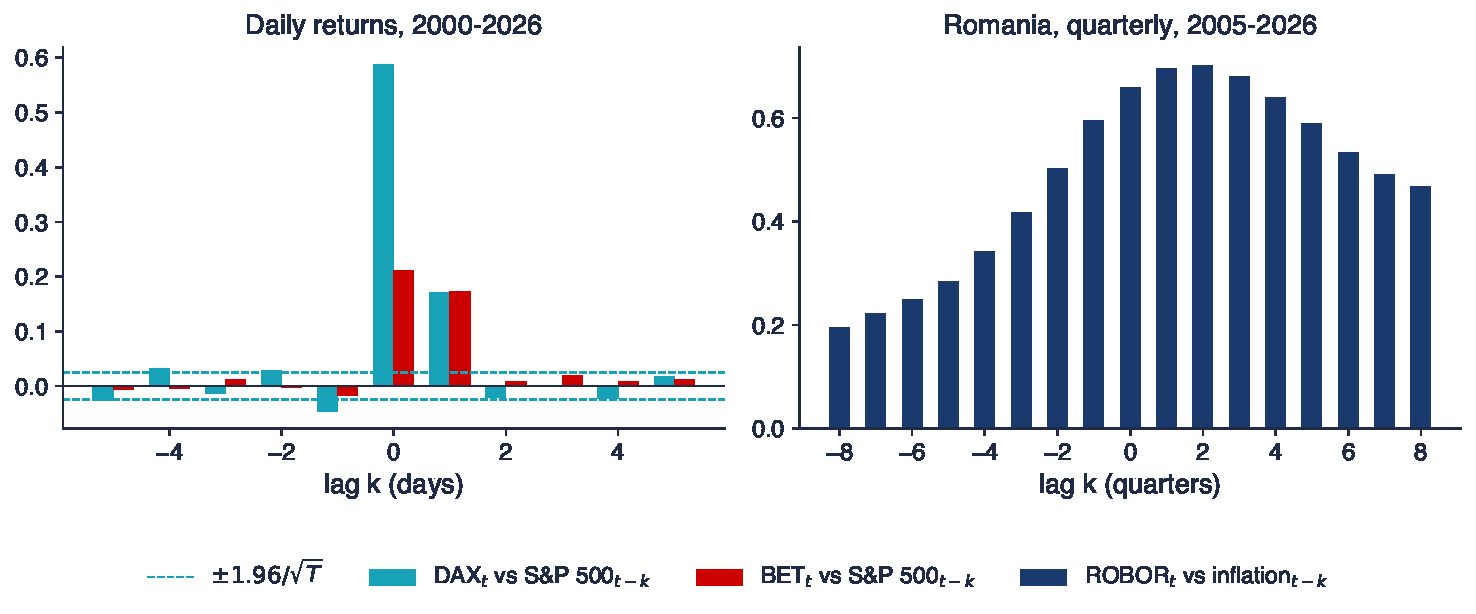
\includegraphics[width=0.97\textwidth,height=0.56\textheight,keepaspectratio]{tsa_ch6_ccf.pdf}
\end{center}
\vspace{-0.25cm}
\begin{itemize}
    \item Left: daily log returns (EODHD), 6\,433 common trading days, 2000--2026; bars: $\Corr(\text{DAX}_t, \text{S\&P}_{t-k})$ and $\Corr(\text{BET}_t, \text{S\&P}_{t-k})$. Right: quarterly ROBOR 3M against lags of inflation
\end{itemize}
\quantlet{TSA\_ch6\_multivariate\_data}{\qlurl{TSA_ch6_multivariate_data}}
\end{frame}

\begin{frame}{Interpreting the cross-correlations}
\itemsize{\small}
\begin{itemize}
    \item BET with the S\&P 500: 0.21 on the same day and 0.17 with the previous day ($k = 1$); with $k = -1$: $-$0.02
    \begin{itemize}
        \item the band is $\pm$0.024: yesterday's New York return is visible in today's Bucharest and Frankfurt returns, not the reverse
        \item reason: Wall Street closes at 22:00 in Frankfurt, after the European markets; its news reaches them the next morning
    \end{itemize}
    \item ROBOR with inflation: the largest correlation, 0.70, is at $k = 2$ quarters (inflation leads)
    \begin{itemize}
        \item but every value is large (0.34 at $k = -4$, 0.64 at $k = 4$): two persistent series; the CCF alone cannot separate lead from persistence
    \end{itemize}
\end{itemize}
\end{frame}

\begin{frame}{The advantage of one model for all series}
\itemsize{\small}
\begin{itemize}
    \item Univariate models (\tsachlink{https://danpele.github.io/Time-Series-Analysis/EN/Courses/chapter2_arma_models.pdf}{Chapters 2}--\tsachlink{https://danpele.github.io/Time-Series-Analysis/EN/Courses/chapter3_unit_roots_arima_models.pdf}{3}) forecast each series from its own past
    \begin{itemize}
        \item they ignore that last quarter's inflation may help to forecast this quarter's interest rate
    \end{itemize}
    \item \textbf{Feedback}: the central bank reacts to inflation, inflation reacts to the interest rate
    \begin{itemize}
        \item a single regression of $\pi_t$ on $i_t$ treats $i_t$ as given (exogenous); here both are \textbf{endogenous}, determined inside the system
    \end{itemize}
    \item A VAR treats all variables symmetrically: each depends on the past of all
    \begin{itemize}
        \item no economic theory is needed to write it down; theory comes back when we interpret shocks (Section 7)
    \end{itemize}
\end{itemize}
\end{frame}

\begin{frame}{Recap: From one series to several}
\itemsize{\small}
\begin{itemize}
    \item A vector series $\bY_t$ has a mean vector and autocovariance matrices $\bGamma(h)$, with $\bGamma(-h) = \bGamma(h)'$
    \item The CCF $\rho_{yx}(k)$ shows lead--lag patterns; $k > 0$: $x$ leads
    \item S\&P 500 returns lead DAX and BET returns by one day
    \item Feedback between variables calls for a joint model
\end{itemize}
\end{frame}


%=============================================================================
\section{The VAR$(p)$ model}
%=============================================================================

\begin{frame}{The VAR$(p)$ model}
\itemsize{\small}
\begin{itemize}
    \item \textbf{Definition}: $\bY_t = \bc + \bA_1\bY_{t-1} + \dots + \bA_p\bY_{t-p} + \bepsilon_t$
    \begin{itemize}
        \item $\bc$: $K \times 1$ vector of constants; $\bA_1, \dots, \bA_p$: $K \times K$ coefficient matrices
        \item $\bepsilon_t$: vector white noise: $E[\bepsilon_t] = \mathbf{0}$, $E[\bepsilon_t\bepsilon_t'] = \bSigma$, $E[\bepsilon_t\bepsilon_s'] = \mathbf{0}$ for $t \ne s$
    \end{itemize}
    \item $\bSigma$ is not diagonal in general: shocks of different equations are correlated \textbf{at the same date}
    \begin{itemize}
        \item no lagged errors are correlated: all the dynamics is in the matrices $\bA_j$
    \end{itemize}
    \item With $K = 1$ we recover the AR$(p)$ of \tsachlink{https://danpele.github.io/Time-Series-Analysis/EN/Courses/chapter2_arma_models.pdf}{Chapter 2}
    \begin{itemize}
        \item this form is called the \textbf{reduced form}: it describes the data, not the economic shocks (Section 10)
    \end{itemize}
\end{itemize}
\end{frame}

\begin{frame}{A bivariate VAR(1), equation by equation}
\itemsize{\small}
\begin{itemize}
    \item In matrix form:
    \begin{itemize}
        \item $\begin{pmatrix} y_{1t} \\ y_{2t} \end{pmatrix} = \begin{pmatrix} c_1 \\ c_2 \end{pmatrix} + \begin{pmatrix} a_{11} & a_{12} \\ a_{21} & a_{22} \end{pmatrix}\begin{pmatrix} y_{1,t-1} \\ y_{2,t-1} \end{pmatrix} + \begin{pmatrix} \varepsilon_{1t} \\ \varepsilon_{2t} \end{pmatrix}$
    \end{itemize}
    \item Equation by equation:
    \begin{itemize}
        \item $y_{1t} = c_1 + a_{11}y_{1,t-1} + a_{12}y_{2,t-1} + \varepsilon_{1t}$
        \item $y_{2t} = c_2 + a_{21}y_{1,t-1} + a_{22}y_{2,t-1} + \varepsilon_{2t}$
    \end{itemize}
    \item Reading the coefficients: $a_{jk}$ = effect of $y_{k,t-1}$ on $y_{jt}$ (row: equation; column: regressor)
    \begin{itemize}
        \item $a_{12} = a_{21} = 0$: two separate AR(1) models; $a_{12} \ne 0$: the past of $y_2$ helps to predict $y_1$
    \end{itemize}
\end{itemize}
\end{frame}

\begin{frame}{Worked example: a VAR(1)}
\itemsize{\small}
\begin{itemize}
    \item Model: $\bc = (1.2, 0.6)'$, $\bA = \begin{pmatrix} 0.5 & 0.2 \\ 0.3 & 0.4 \end{pmatrix}$, $\bSigma = \begin{pmatrix} 1 & 0.5 \\ 0.5 & 1 \end{pmatrix}$
    \begin{itemize}
        \item $y_{1t} = 1.2 + 0.5y_{1,t-1} + 0.2y_{2,t-1} + \varepsilon_{1t}$; \quad $y_{2t} = 0.6 + 0.3y_{1,t-1} + 0.4y_{2,t-1} + \varepsilon_{2t}$
    \end{itemize}
    \item Reading: $a_{21} = 0.3$: one unit more of $y_1$ last period raises $y_2$ by 0.3 today, other things fixed
    \begin{itemize}
        \item the shocks are correlated: $\Corr(\varepsilon_{1t}, \varepsilon_{2t}) = 0.5$
    \end{itemize}
    \item Forecasts from $\bY_T = (5, 2)'$: $\hat\bY_{T+1} = \bc + \bA\bY_T = \begin{pmatrix} 4.10 \\ 2.90 \end{pmatrix}$, \quad $\hat\bY_{T+2} = \bc + \bA\hat\bY_{T+1} = \begin{pmatrix} 3.83 \\ 2.99 \end{pmatrix}$
    \begin{itemize}
        \item the forecasts move towards the mean $\boldsymbol{\mu} = (3.50, 2.75)'$ (next section)
    \end{itemize}
\end{itemize}
\end{frame}

\begin{frame}{The worked example, simulated}
\itemsize{\footnotesize}
\begin{center}
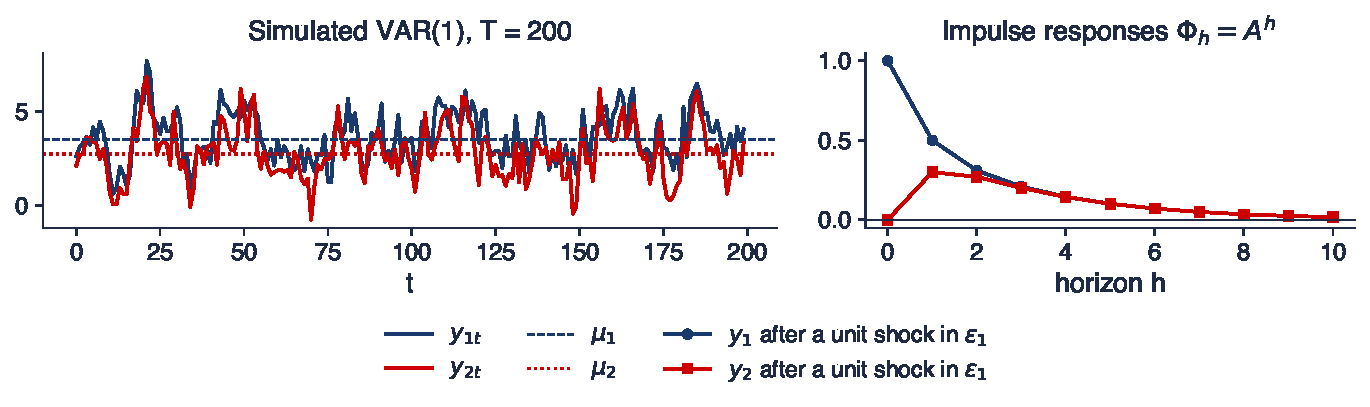
\includegraphics[width=0.97\textwidth,height=0.56\textheight,keepaspectratio]{tsa_ch6_var_sim.pdf}
\end{center}
\vspace{-0.25cm}
\begin{itemize}
    \item Left: 200 periods of the VAR(1) of the previous slide, with its two means; right: the responses of $y_1$ and $y_2$ to a unit shock in $\varepsilon_1$ at $h = 0$, the columns of $\bA^h$
\end{itemize}
\quantlet{TSA\_ch6\_var\_stability}{\qlurl{TSA_ch6_var_stability}}
\end{frame}

\begin{frame}{Interpreting the simulated VAR(1)}
\itemsize{\small}
\begin{itemize}
    \item The two series wander around their means and move together: sample correlation 0.75
    \begin{itemize}
        \item two sources of co-movement: the correlated shocks ($\Corr = 0.5$) and the cross effects $a_{12}$, $a_{21}$
    \end{itemize}
    \item A unit shock to $y_1$ reaches $y_2$ one period later ($a_{21} = 0.3$), then both fade
    \begin{itemize}
        \item the decay is governed by the largest eigenvalue of $\bA$, 0.7: after 5 periods about $0.7^5 \approx 0.17$ of the effect remains
    \end{itemize}
\end{itemize}
\end{frame}

\begin{frame}{The number of parameters}
\itemsize{\small}
\begin{itemize}
    \item A VAR$(p)$ with $K$ variables and a constant: $K + pK^2$ coefficients, plus $K(K+1)/2$ in $\bSigma$
    \begin{itemize}
        \item each equation has $1 + pK$ regressors
        \item Romanian VAR: $K = 3$, $p = 2$: $3 + 2 \cdot 9 = 21$ coefficients estimated on 84 quarters
    \end{itemize}
    \item \textbf{The curse of dimensionality}: $K = 5$, $p = 4$: $5 + 4 \cdot 25 = 105$ coefficients
    \begin{itemize}
        \item with 25 years of quarterly data (100 observations) each equation has 21 regressors and 79 residual degrees of freedom
    \end{itemize}
    \item Hence small VARs (3--6 variables), few lags, and estimates with large standard errors; individual coefficients are rarely interpreted
\end{itemize}
\end{frame}

\begin{frame}{Christopher Sims and "Macroeconomics and Reality"}
\itemsize{\small}
\begin{columns}[T]
\begin{column}{0.38\textwidth}
\centering

\includegraphics[height=0.56\textheight]{ch6_christopher_sims_2011.jpg}\\[1mm]
\imgcap{Christopher A. Sims, Nobel Prize in Economics 2011}
\imgcredit{https://commons.wikimedia.org/wiki/File:Christopher_A._Sims_close-up_(cropped).jpg}{Photo: Holger Motzkau (2011); CC BY-SA 3.0; Wikimedia Commons}
\end{column}
\begin{column}{0.6\textwidth}
\begin{itemize}
    \item \refSims: the large macro models of the 1970s imposed ``incredible'' restrictions
    \begin{itemize}
        \item which variables are exogenous, which lags are zero
        \item his proposal: an unrestricted VAR that lets the data speak
        \item then only the few assumptions needed to interpret the shocks
    \end{itemize}
    \item The VAR became the standard tool of central banks for forecasting and for measuring the effects of monetary policy
    \item Nobel Prize 2011, with Thomas Sargent, ``for their empirical research on cause and effect in the macroeconomy''
\end{itemize}
\end{column}
\end{columns}
\end{frame}

\begin{frame}{Recap: The VAR$(p)$ model}
\itemsize{\small}
\begin{itemize}
    \item $\bY_t = \bc + \sum_{j=1}^{p}\bA_j\bY_{t-j} + \bepsilon_t$, $\bepsilon_t$ white noise with covariance $\bSigma$
    \item $a_{jk}$: effect of the lag of variable $k$ in the equation of variable $j$
    \item $K + pK^2$ coefficients: keep $K$ and $p$ small
    \item \refSims: VARs as an alternative to ``incredible'' restrictions
\end{itemize}
\end{frame}


%=============================================================================
\section{Stationarity and the companion form}
%=============================================================================

\begin{frame}{Stability of a VAR(1)}
\itemsize{\small}
\begin{itemize}
    \item Substitute repeatedly: $\bY_t = \bc + \bA\bc + \dots + \bA^{h-1}\bc + \bA^h\bY_{t-h} + \sum_{j=0}^{h-1}\bA^j\bepsilon_{t-j}$
    \begin{itemize}
        \item the past is forgotten only if $\bA^h \to \mathbf{0}$
    \end{itemize}
    \item \textbf{Stability condition}: all eigenvalues $\lambda$ of $\bA$ satisfy $|\lambda| < 1$
    \begin{itemize}
        \item eigenvalues: the roots of $\det(\bA - \lambda\mathbf{I}) = 0$; for $K = 2$: $\lambda^2 - \mathrm{tr}(\bA)\lambda + \det(\bA) = 0$
        \item $\mathbf{I}$: the identity matrix; $\mathrm{tr}(\bA) = a_{11} + a_{22}$: the trace; $\det(\bA) = a_{11}a_{22} - a_{12}a_{21}$: the determinant; $|\lambda|$: the modulus (eigenvalues can be complex)
        \item a stable VAR is weakly stationary (if it started long ago); this is the multivariate version of $|\phi| < 1$ (\tsachlink{https://danpele.github.io/Time-Series-Analysis/EN/Courses/chapter2_arma_models.pdf}{Chapter 2})
    \end{itemize}
    \item \textbf{Example}: $\mathrm{tr}(\bA) = 0.9$, $\det(\bA) = 0.5 \cdot 0.4 - 0.2 \cdot 0.3 = 0.14$: $\lambda^2 - 0.9\lambda + 0.14 = 0$
    \begin{itemize}
        \item $\lambda = (0.9 \pm 0.5)/2$: $\lambda_1 = 0.7$, $\lambda_2 = 0.2$; both inside the unit circle: stable
    \end{itemize}
\end{itemize}
\end{frame}

\begin{frame}{Mean and variance of a stable VAR(1)}
\itemsize{\small}
\begin{itemize}
    \item \textbf{Mean}: take expectations, $\boldsymbol{\mu} = \bc + \bA\boldsymbol{\mu}$, so $\boldsymbol{\mu} = (\mathbf{I} - \bA)^{-1}\bc$
    \begin{itemize}
        \item example: $\mathbf{I} - \bA = \begin{pmatrix} 0.5 & -0.2 \\ -0.3 & 0.6 \end{pmatrix}$, determinant 0.24; $\boldsymbol{\mu} = \frac{1}{0.24}\begin{pmatrix} 0.6 & 0.2 \\ 0.3 & 0.5 \end{pmatrix}\begin{pmatrix} 1.2 \\ 0.6 \end{pmatrix} = \begin{pmatrix} 3.50 \\ 2.75 \end{pmatrix}$
    \end{itemize}
    \item \textbf{Variance}: $\bGamma(0) = \bA\bGamma(0)\bA' + \bSigma$ (a discrete Lyapunov equation); $\bGamma(h) = \bA^h\bGamma(0)$
    \begin{itemize}
        \item solved by $\mathrm{vec}\,\bGamma(0) = (\mathbf{I} - \bA \otimes \bA)^{-1}\mathrm{vec}\,\bSigma$; example: $\bGamma(0) = \begin{pmatrix} 1.75 & 1.22 \\ 1.22 & 1.73 \end{pmatrix}$
        \item $\otimes$: the Kronecker product; $\mathrm{vec}$ stacks the columns of a matrix
    \end{itemize}
    \item The variances 1.75 and 1.73 exceed those of the shocks (1): the dynamics accumulates past shocks
\end{itemize}
\end{frame}

\begin{frame}{The companion form of a VAR$(p)$}
\itemsize{\small}
\begin{itemize}
    \item Stack $p$ consecutive vectors: $\boldsymbol{\xi}_t = (\bY_t', \bY_{t-1}', \dots, \bY_{t-p+1}')'$, of size $Kp$
    \begin{itemize}
        \item then $\boldsymbol{\xi}_t = \boldsymbol{\nu} + \mathbf{F}\boldsymbol{\xi}_{t-1} + \mathbf{v}_t$: every VAR$(p)$ is a VAR(1) in $\boldsymbol{\xi}_t$
        \item $\boldsymbol{\nu}$: $\bc$ followed by zeros; $\mathbf{v}_t$: $\bepsilon_t$ followed by zeros; $\mathbf{F}$: the $Kp \times Kp$ companion matrix
    \end{itemize}
    \item For $p = 2$: $\begin{pmatrix} \bY_t \\ \bY_{t-1} \end{pmatrix} = \begin{pmatrix} \bc \\ \mathbf{0} \end{pmatrix} + \underbrace{\begin{pmatrix} \bA_1 & \bA_2 \\ \mathbf{I}_K & \mathbf{0} \end{pmatrix}}_{\mathbf{F}}\begin{pmatrix} \bY_{t-1} \\ \bY_{t-2} \end{pmatrix} + \begin{pmatrix} \bepsilon_t \\ \mathbf{0} \end{pmatrix}$
    \begin{itemize}
        \item the second block row is the identity $\bY_{t-1} = \bY_{t-1}$
    \end{itemize}
    \item \textbf{Stability of a VAR$(p)$}: all $Kp$ eigenvalues of the companion matrix $\mathbf{F}$ have modulus below 1
    \begin{itemize}
        \item equivalently: all roots $z$ (complex numbers) of $\det(\mathbf{I}_K - \bA_1z - \dots - \bA_pz^p) = 0$ lie outside the unit circle
        \item the eigenvalues of $\bA_1$ alone say nothing about the stability of a VAR(2)
    \end{itemize}
\end{itemize}
\end{frame}

\begin{frame}{Eigenvalues of three estimated VARs}
\itemsize{\footnotesize}
\begin{center}
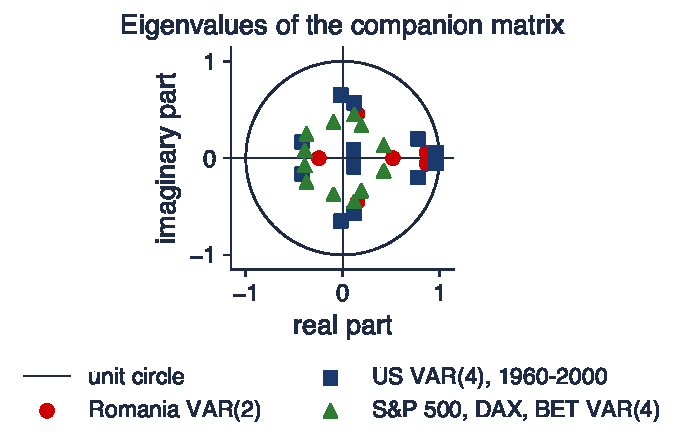
\includegraphics[width=0.97\textwidth,height=0.6\textheight,keepaspectratio]{tsa_ch6_roots.pdf}
\end{center}
\vspace{-0.25cm}
\begin{itemize}
    \item Companion matrices: Romanian VAR(2) (GDP growth, inflation, ROBOR 3M; 6 eigenvalues), the US VAR(4) of Section 10 (12), the daily S\&P 500, DAX and BET VAR(4) (12)
\end{itemize}
\quantlet{TSA\_ch6\_var\_stability}{\qlurl{TSA_ch6_var_stability}}
\end{frame}

\begin{frame}{Interpreting the eigenvalues}
\itemsize{\small}
\begin{itemize}
    \item All three VARs are stable; largest moduli: Romania 0.869, US 0.969, markets 0.464
    \begin{itemize}
        \item the largest modulus sets the speed at which shocks fade: $0.97^{20} \approx 0.54$ after 20 quarters, $0.46^{2} \approx 0.21$ after 2 days
    \end{itemize}
    \item Macro VARs have eigenvalues close to 1 (persistent inflation and interest rates); return VARs have small ones
    \begin{itemize}
        \item complex pairs produce damped oscillations in the responses
    \end{itemize}
    \item An eigenvalue very close to 1 signals a unit root, perhaps cointegration: \tsachlink{https://danpele.github.io/Time-Series-Analysis/EN/Courses/chapter7_cointegration_vecm.pdf}{Chapter 7}
\end{itemize}
\end{frame}

\begin{frame}{The moving-average representation}
\itemsize{\small}
\begin{itemize}
    \item A stable VAR can be written as an infinite moving average of the shocks (Wold, \tsachlink{https://danpele.github.io/Time-Series-Analysis/EN/Courses/chapter1_stochastic_processes_stationarity.pdf}{Chapter 1}):
    \begin{itemize}
        \item $\bY_t = \boldsymbol{\mu} + \bepsilon_t + \bPhi_1\bepsilon_{t-1} + \bPhi_2\bepsilon_{t-2} + \dots = \boldsymbol{\mu} + \sum_{h=0}^{\infty}\bPhi_h\bepsilon_{t-h}$, $\bPhi_0 = \mathbf{I}$
        \item $\bPhi_h$: the $K \times K$ matrix that weights the shock of $h$ periods ago
    \end{itemize}
    \item VAR(1): $\bPhi_h = \bA^h$; VAR$(p)$: $\bPhi_h = \sum_{j=1}^{\min(h,p)}\bA_j\bPhi_{h-j}$
    \begin{itemize}
        \item example: $\bPhi_2 = \bA^2 = \begin{pmatrix} 0.31 & 0.18 \\ 0.27 & 0.22 \end{pmatrix}$
    \end{itemize}
    \item Element $(j, k)$ of $\bPhi_h$: the effect on $Y_{j,t+h}$ of a unit change in $\varepsilon_{kt}$, all other shocks fixed
    \begin{itemize}
        \item these are the \textbf{impulse responses} (Section 7); they also give the forecast errors (Sections 8--9)
    \end{itemize}
\end{itemize}
\end{frame}

\begin{frame}{Recap: Stationarity and the companion form}
\itemsize{\small}
\begin{itemize}
    \item VAR(1): stable if all eigenvalues of $\bA$ have $|\lambda| < 1$; VAR$(p)$: the same for the companion matrix
    \item Mean $\boldsymbol{\mu} = (\mathbf{I} - \bA_1 - \dots - \bA_p)^{-1}\bc$; forecasts converge to it
    \item Moving-average form $\bY_t = \boldsymbol{\mu} + \sum_h\bPhi_h\bepsilon_{t-h}$: the basis of impulse responses
    \item Estimated macro VARs have eigenvalues close to 1
\end{itemize}
\end{frame}


%=============================================================================
\section{Estimation and lag selection}
%=============================================================================

\begin{frame}{Estimation by OLS, equation by equation}
\itemsize{\small}
\begin{itemize}
    \item Each equation is a linear regression of $Y_{jt}$ on a constant and $\bY_{t-1}, \dots, \bY_{t-p}$
    \begin{itemize}
        \item the same $1 + Kp$ regressors in every equation; OLS (ordinary least squares) on each equation separately
    \end{itemize}
    \item \textbf{OLS is enough}: with identical regressors, system estimation (GLS, generalised least squares, on all equations) gives exactly the OLS estimates
    \begin{itemize}
        \item the correlation of the shocks does not improve the estimates; under Normal errors OLS is also the maximum likelihood estimator
    \end{itemize}
    \item \textbf{Covariance of the shocks}: $\hat\bSigma = \frac{1}{T - Kp - 1}\sum_t\hat\bepsilon_t\hat\bepsilon_t'$, from the residuals of all equations
    \begin{itemize}
        \item $\hat\bepsilon_t$: the vector of residuals at date $t$; $T - Kp - 1$: the residual degrees of freedom of each equation
        \item stationarity matters: with stationary series the usual $t$ and $F$ tests are valid in large samples
    \end{itemize}
\end{itemize}
\end{frame}

\begin{frame}{Choosing $p$: information criteria}
\itemsize{\small}
\begin{itemize}
    \item Fit VAR$(p)$ for $p = 0, \dots, p_{\max}$ on the \textbf{same sample}; $\tilde\bSigma(p)$: residual covariance divided by $T$
    \begin{itemize}
        \item AIC (Akaike) $= \ln\det\tilde\bSigma(p) + \frac{2}{T}pK^2$ \refAkaike
        \item BIC (Schwarz) $= \ln\det\tilde\bSigma(p) + \frac{\ln T}{T}pK^2$ \refSchwarz
        \item HQ (Hannan--Quinn) $= \ln\det\tilde\bSigma(p) + \frac{2\ln\ln T}{T}pK^2$ \refHQ
        \item $\det\tilde\bSigma(p)$: a generalised residual variance; $pK^2$: the number of lag coefficients; $p_{\max}$: the largest order tried
    \end{itemize}
    \item First term: fit (smaller residual ``volume''); second: a penalty per coefficient; choose the $p$ with the smallest value
    \begin{itemize}
        \item penalties: AIC $<$ HQ $<$ BIC (for $T \ge 16$): BIC chooses the smallest $p$, AIC the largest
        \item BIC and HQ are consistent (they find the true $p$ as $T \to \infty$); AIC tends to overfit, but often forecasts well
    \end{itemize}
\end{itemize}
\end{frame}

\begin{frame}{Romanian VAR: which $p$?}
\itemsize{\footnotesize}
\begin{center}
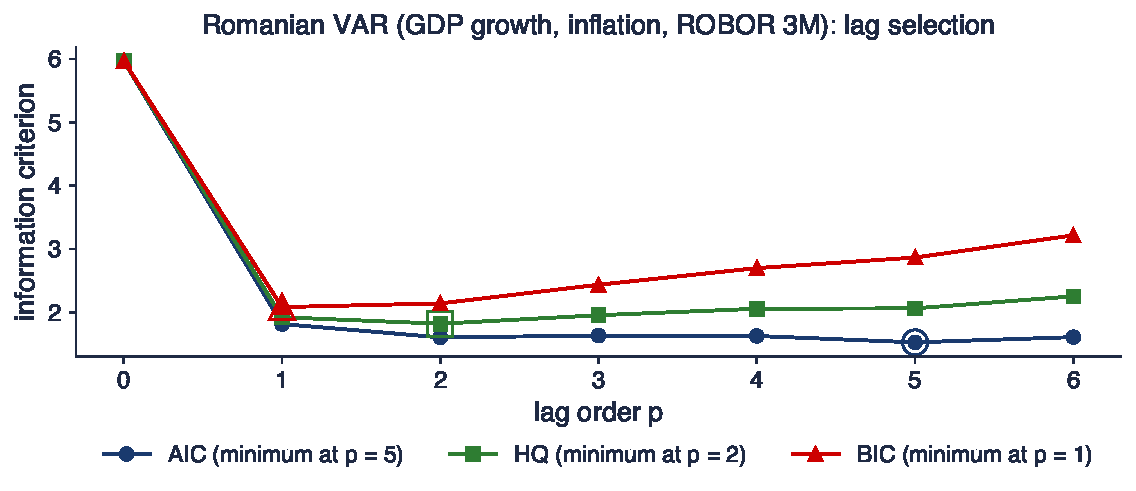
\includegraphics[width=0.97\textwidth,height=0.56\textheight,keepaspectratio]{tsa_ch6_ic.pdf}
\end{center}
\vspace{-0.25cm}
\begin{itemize}
    \item GDP growth, 12-month inflation and ROBOR 3M, 2005Q1--2026Q2; VAR$(p)$ for $p = 0, \dots, 6$ on the common sample of 80 quarters; circles mark the minima
\end{itemize}
\quantlet{TSA\_ch6\_estimation\_diagnostics}{\qlurl{TSA_ch6_estimation_diagnostics}}
\end{frame}

\begin{frame}{Interpreting the lag selection}
\itemsize{\small}
\begin{itemize}
    \item BIC chooses $p = 1$, HQ $p = 2$, AIC $p = 5$: the three criteria disagree, as they often do in short samples
    \begin{itemize}
        \item AIC: 1.812 at $p = 1$, 1.603 at $p = 2$, 1.523 at $p = 5$: a flat curve after $p = 2$
    \end{itemize}
    \item $p = 5$ would mean $3 + 5 \cdot 9 = 48$ coefficients for about 80 quarters
    \begin{itemize}
        \item we take $p = 2$ (HQ), then check whether the residuals are white noise; if not, we add lags
    \end{itemize}
    \item A rule of thumb: start from the criteria, never stop at them
\end{itemize}
\end{frame}

\begin{frame}{The estimated Romanian VAR(2)}
\itemsize{\small}
\begin{center}
\scriptsize
\begin{tabular}{lrrr}
\toprule
\textbf{Regressor} & \textbf{equation $g_t$} & \textbf{equation $\pi_t$} & \textbf{equation $i_t$} \\
\midrule
constant & $1.09$ ($2.1$) & $0.49$ ($2.0$) & $-0.11$ ($-0.6$) \\
$g_{t-1}$ & $0.01$ ($0.1$) & $0.01$ ($0.1$) & $0.14$ ($3.5$) \\
$\pi_{t-1}$ & $0.53$ ($2.3$) & $1.26$ ($11.7$) & $0.24$ ($2.8$) \\
$i_{t-1}$ & $-0.73$ ($-2.7$) & $0.16$ ($1.2$) & $1.04$ ($10.2$) \\
$g_{t-2}$ & $-0.08$ ($-0.7$) & $-0.03$ ($-0.5$) & $0.07$ ($1.7$) \\
$\pi_{t-2}$ & $-0.41$ ($-1.7$) & $-0.35$ ($-3.1$) & $-0.17$ ($-1.9$) \\
$i_{t-2}$ & $0.54$ ($2.0$) & $-0.16$ ($-1.3$) & $-0.12$ ($-1.2$) \\
$R^2$ & 0.16 & 0.90 & 0.93 \\
\bottomrule
\end{tabular}
\end{center}
\begin{itemize}
    \item OLS on 84 quarters (2005Q3--2026Q2); $t$-statistics in parentheses; 21 coefficients
    \item Residual standard deviations: 2.32 ($g$), 1.09 ($\pi$), 0.87 ($i$); residual correlation of $\pi$ and $i$: 0.25
\end{itemize}
\end{frame}

\begin{frame}{Interpreting the coefficients}
\itemsize{\small}
\begin{itemize}
    \item Inflation is very persistent: $1.26\,\pi_{t-1} -0.35\,\pi_{t-2}$; ROBOR too: $1.04\,i_{t-1}$
    \begin{itemize}
        \item $R^2$ of 0.90 and 0.93: most of it is the series' own past
    \end{itemize}
    \item In the ROBOR equation, past GDP growth ($t = 3.5$) and past inflation ($t = 2.8$) matter: the interest rate follows the economy
    \begin{itemize}
        \item GDP growth is hard to predict: $R^2 = 0.16$
    \end{itemize}
    \item Single coefficients of correlated lags are unstable (e.g.\ $i_{t-1}$ and $i_{t-2}$ with opposite signs in the $g$ equation): read the system through tests, responses and forecasts, not one coefficient at a time
\end{itemize}
\end{frame}

\begin{frame}{Recap: Estimation and lag selection}
\itemsize{\small}
\begin{itemize}
    \item OLS equation by equation is efficient: all equations have the same regressors
    \item AIC, BIC, HQ: $\ln\det\tilde\bSigma(p)$ plus a penalty; compare on a common sample
    \item BIC $\le$ HQ $\le$ AIC in the chosen $p$; Romanian VAR: $p = 2$
    \item Interpret the system, not single coefficients
\end{itemize}
\end{frame}


%=============================================================================
\section{Residual diagnostics}
%=============================================================================

\begin{frame}{Are the residuals white noise?}
\itemsize{\small}
\begin{itemize}
    \item \textbf{Multivariate portmanteau test} \refHosking
    \begin{itemize}
        \item $H_0$: no autocorrelation and no cross-correlation of the residuals up to lag $h$
        \item $Q_h = T^2\sum_{j=1}^{h}\frac{1}{T - j}\mathrm{tr}(\hat{\mathbf{C}}_j'\hat{\mathbf{C}}_0^{-1}\hat{\mathbf{C}}_j\hat{\mathbf{C}}_0^{-1})$, $\hat{\mathbf{C}}_j = \frac{1}{T}\sum_t\hat\bepsilon_t\hat\bepsilon_{t-j}'$: the residual autocovariance matrix at lag $j$; $\mathrm{tr}$: the trace
        \item under $H_0$: $\chi^2$ with $K^2(h - p)$ degrees of freedom; the multivariate Ljung--Box test (\tsachlink{https://danpele.github.io/Time-Series-Analysis/EN/Courses/chapter2_arma_models.pdf}{Chapter 2}); a small p-value: the residuals are still autocorrelated
    \end{itemize}
    \item \textbf{Normality}: a multivariate Jarque--Bera test \refJB\ on the standardised residuals (skewness and kurtosis)
    \begin{itemize}
        \item Normality is not needed for OLS; it matters for exact intervals and for small samples
    \end{itemize}
    \item If the portmanteau test rejects: add lags, add a variable, or model breaks and outliers (dummy variables)
    \begin{itemize}
        \item also check stability (eigenvalues) and, for long samples, parameter stability over time
    \end{itemize}
\end{itemize}
\end{frame}

\begin{frame}{Residuals of the Romanian VAR(2)}
\itemsize{\footnotesize}
\begin{center}
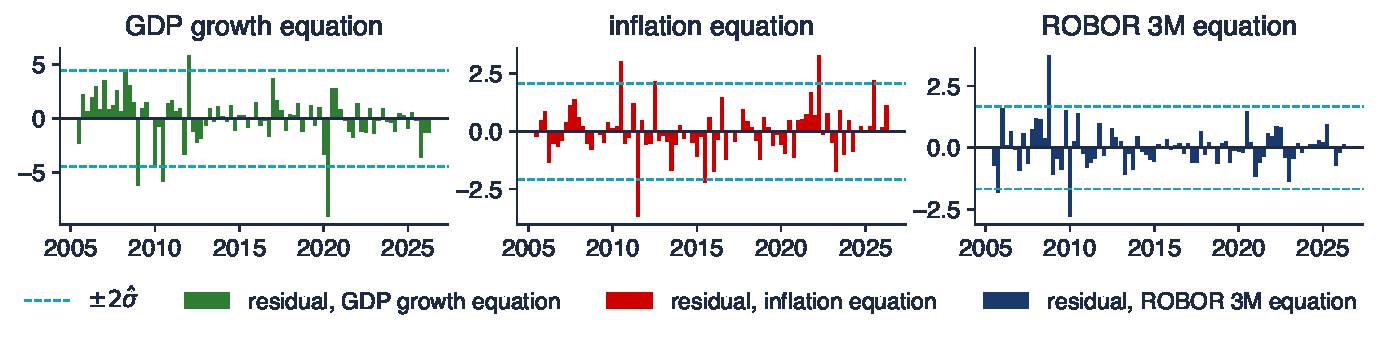
\includegraphics[width=0.97\textwidth,height=0.5\textheight,keepaspectratio]{tsa_ch6_resid.pdf}
\end{center}
\vspace{-0.25cm}
\begin{itemize}
    \item Residuals of the three equations, 2005Q3--2026Q2, with $\pm 2$ residual standard deviations
\end{itemize}
\quantlet{TSA\_ch6\_estimation\_diagnostics}{\qlurl{TSA_ch6_estimation_diagnostics}}
\end{frame}

\begin{frame}{Interpreting the residuals}
\itemsize{\small}
\begin{itemize}
    \item Largest residuals: GDP $-$9.1 in 2020Q2 (the pandemic), ROBOR $+3.7$ in 2008Q4 (the 2008 liquidity squeeze), inflation $-$3.7 in 2011Q3
    \begin{itemize}
        \item kurtosis 6.5 ($g$) and 7.9 ($i$), against 3 under the Normal distribution: Jarque--Bera 191 (p $<$\,0.001)
    \end{itemize}
    \item Portmanteau: $Q_8 = 76.7$ ($54$ d.f., p = 0.023); $Q_{12} = 105.3$ ($90$ d.f., p = 0.130)
    \begin{itemize}
        \item borderline at 8 lags, fine at 12: some short-run correlation is left, partly from overlapping 12-month inflation rates
    \end{itemize}
    \item Consequence: point estimates are usable, but the intervals of the next sections rely on large-sample approximations; we use bootstrap bands for the responses
\end{itemize}
\end{frame}

\begin{frame}{Recap: Residual diagnostics}
\itemsize{\small}
\begin{itemize}
    \item Portmanteau test: $H_0$ white-noise residuals, $\chi^2$ with $K^2(h - p)$ d.f.
    \item Normality fails in macro data: crises produce outliers
    \item Remedies: more lags, more variables, dummies for crisis quarters
\end{itemize}
\end{frame}


%=============================================================================
\section{Granger causality}
%=============================================================================

\begin{frame}{Granger causality: the definition}
\itemsize{\small}
\begin{columns}[T]
\begin{column}{0.3\textwidth}
\centering
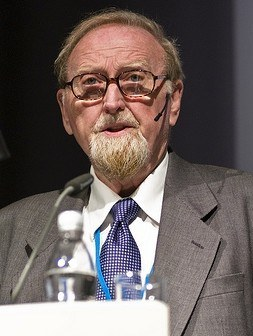
\includegraphics[height=0.44\textheight]{ch3_clive_granger_2008.jpg}\\[1mm]
\imgcap{Clive Granger (1934--2009), Nobel Prize in Economics 2003}
\imgcredit{https://commons.wikimedia.org/wiki/File:Clive_Granger_by_Olaf_Storbeck_(3x4_cropped).jpg}{Photo: Olaf Storbeck (2008); CC BY-SA 2.0; Wikimedia Commons}
\end{column}
\begin{column}{0.68\textwidth}
\begin{itemize}
    \item \textbf{Definition} \refGranger: $x$ \textbf{Granger-causes} $y$
    \begin{itemize}
        \item if the past of $x$ improves the forecast of $y$ made from the past of $y$ (and of the other variables)
        \item formally: the MSE (mean squared error) of the optimal forecast of $y_{t+1}$ is smaller when $x_t, x_{t-1}, \dots$ are used
    \end{itemize}
    \item A statement about \textbf{predictability}, not about cause and effect
    \begin{itemize}
        \item the cause comes before the effect, but ``before'' does not imply ``because''
    \end{itemize}
    \item Four cases: no causality, $x \to y$, $y \to x$, feedback $x \leftrightarrow y$
\end{itemize}
\end{column}
\end{columns}
\end{frame}

\begin{frame}{Testing Granger causality in a VAR}
\itemsize{\small}
\begin{itemize}
    \item In a VAR$(p)$, $x$ does not Granger-cause $y$ if all coefficients of $x_{t-1}, \dots, x_{t-p}$ in the equation of $y$ are zero
    \begin{itemize}
        \item bivariate VAR(2): $H_0$: $a_{12}^{(1)} = a_{12}^{(2)} = 0$ in $y_t = c + a_{11}^{(1)}y_{t-1} + a_{12}^{(1)}x_{t-1} + a_{11}^{(2)}y_{t-2} + a_{12}^{(2)}x_{t-2} + \varepsilon_t$
        \item $a_{12}^{(j)}$: the coefficient of $x_{t-j}$ in the equation of $y$ (the superscript is the lag)
    \end{itemize}
    \item \textbf{$F$ test}: $F = \dfrac{(RSS_R - RSS_U)/p}{RSS_U/(T - Kp - 1)} \sim F(p, T - Kp - 1)$ under $H_0$
    \begin{itemize}
        \item $RSS_U$: residual sum of squares of the equation of $y$; $RSS_R$: the same without the lags of $x$
        \item a large $F$ (a small p-value): dropping the lags of $x$ raises the RSS too much, so $H_0$ is rejected
    \end{itemize}
    \item \textbf{Wald test}: $W = (\mathbf{R}\hat{\boldsymbol{\beta}})'[\mathbf{R}\hat{\mathbf{V}}\mathbf{R}']^{-1}(\mathbf{R}\hat{\boldsymbol{\beta}}) \sim \chi^2(p)$; here $W = pF$
    \begin{itemize}
        \item $\hat{\boldsymbol{\beta}}$: the estimated coefficients of the equation of $y$; $\mathbf{R}$ selects the tested ones; $\hat{\mathbf{V}}$: the estimated covariance of $\hat{\boldsymbol{\beta}}$; both versions need stationary variables
    \end{itemize}
\end{itemize}
\end{frame}

\begin{frame}{Worked example: does GDP growth Granger-cause ROBOR?}
\itemsize{\small}
\begin{itemize}
    \item Equation of $i_t$ in the Romanian VAR(2), $T = 84$, $K = 3$, $p = 2$
    \begin{itemize}
        \item unrestricted (with $g_{t-1}$, $g_{t-2}$): $RSS_U = 58.27$; restricted (without them): $RSS_R = 69.27$
    \end{itemize}
    \item $F = \dfrac{(69.27 - 58.27)/2}{58.27/77} = \dfrac{5.498}{0.7568} = 7.26$
    \begin{itemize}
        \item degrees of freedom $(2, 84 - 6 - 1) = (2, 77)$; 5\% critical value 3.12; p-value 0.001
    \end{itemize}
    \item \textbf{Decision}: reject $H_0$: past GDP growth helps to forecast ROBOR 3M, given past inflation and past ROBOR
    \begin{itemize}
        \item consistent with a central bank that tightens when the economy grows fast
    \end{itemize}
\end{itemize}
\end{frame}

\begin{frame}{Granger causality in the Romanian VAR(2)}
\itemsize{\small}
\begin{center}
\footnotesize
\begin{tabular}{llrr}
\toprule
\textbf{Cause} & \textbf{Effect} & $F$ & \textbf{p} \\
\midrule
GDP growth & inflation & 0.16 & 0.853 \\
GDP growth & ROBOR 3M & 7.26 & 0.001 \\
inflation & GDP growth & 2.94 & 0.059 \\
inflation & ROBOR 3M & 4.74 & 0.011 \\
ROBOR 3M & GDP growth & 4.02 & 0.022 \\
ROBOR 3M & inflation & 0.89 & 0.417 \\
\bottomrule
\end{tabular}
\end{center}
\begin{itemize}
    \item $F(2, 77)$ tests in the VAR(2), 2005Q3--2026Q2; 5\% critical value 3.12
    \item Significant at 5\%: GDP growth $\to$ ROBOR, inflation $\to$ ROBOR, ROBOR $\to$ GDP growth
\end{itemize}\quantlet{TSA\_ch6\_granger}{\qlurl{TSA_ch6_granger}}
\end{frame}

\begin{frame}{Interpreting the Granger tests}
\itemsize{\small}
\begin{itemize}
    \item The interest rate follows the economy: past growth and past inflation help to forecast ROBOR
    \begin{itemize}
        \item the pattern of a reaction function (the central bank responds to inflation and activity); the test alone cannot prove it is the BNR's rule
    \end{itemize}
    \item ROBOR does not Granger-cause inflation (p = 0.417): no evidence that past rates improve inflation forecasts
    \begin{itemize}
        \item this does not say that monetary policy is ineffective: the effect may be slow, small relative to the noise, or already anticipated
    \end{itemize}
    \item ROBOR $\to$ GDP growth (p = 0.022): higher rates come before weaker growth; in the bivariate VAR (GDP, ROBOR) alone the p-value is 0.063
\end{itemize}
\end{frame}

\begin{frame}{Markets: does New York lead Frankfurt and Bucharest?}
\itemsize{\footnotesize}
\begin{columns}[T]
\begin{column}{0.36\textwidth}
\centering
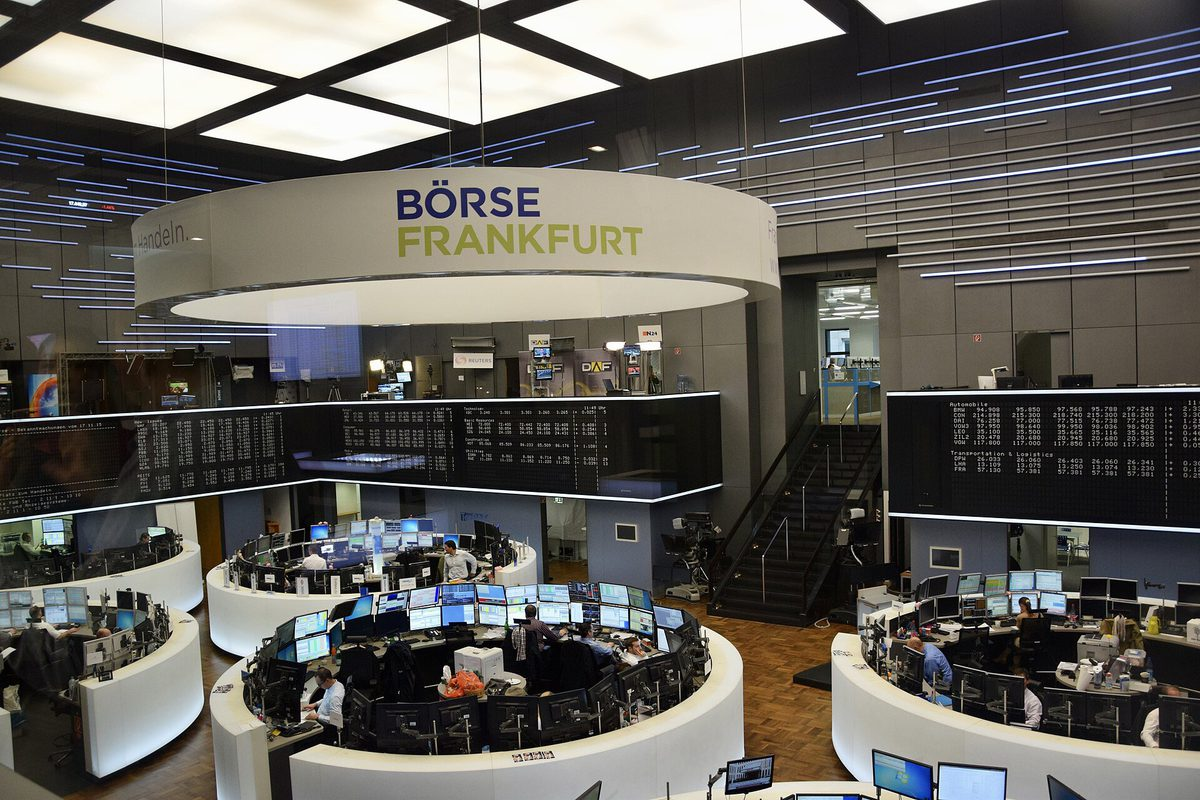
\includegraphics[height=0.34\textheight]{ch6_frankfurt_exchange_2015.jpg}\\[1mm]
\imgcap{Trading floor of the Frankfurt Stock Exchange (DAX)}
\imgcredit{https://commons.wikimedia.org/wiki/File:Frankfurt_Stock_Exchange_(Ank_Kumar)_01.jpg}{Photo: Ank Kumar (2015); CC BY-SA 4.0; Wikimedia Commons}
\end{column}
\begin{column}{0.62\textwidth}
\begin{center}
\scriptsize
\begin{tabular}{llrr}
\toprule
\textbf{Cause} & \textbf{Effect} & $F$ & \textbf{p} \\
\midrule
S\&P 500 & DAX & 94.6 & $<$\,0.001 \\
S\&P 500 & BET & 37.8 & $<$\,0.001 \\
DAX & S\&P 500 & 6.9 & $<$\,0.001 \\
DAX & BET & 3.2 & 0.012 \\
BET & S\&P 500 & 1.0 & 0.416 \\
BET & DAX & 2.6 & 0.032 \\
\bottomrule
\end{tabular}
\end{center}
\begin{itemize}
    \item Daily log returns, VAR(4) (the order of \refDYb), 6\,429 days, 2000--2026; $F(4, \cdot)$ tests; HQ would choose $p = 2$, AIC $p = 8$
    \item Coefficient of the S\&P 500 of yesterday in the BET equation: 0.218 (SE 0.018); in the DAX equation: 0.346
\end{itemize}
\end{column}
\end{columns}
\quantlet{TSA\_ch6\_granger}{\qlurl{TSA_ch6_granger}}
\end{frame}

\begin{frame}{Interpreting the market tests}
\itemsize{\small}
\begin{itemize}
    \item Strong one-way causality from the S\&P 500 to the DAX and the BET: a 1\% S\&P return yesterday adds about 0.218\% to the BET today
    \begin{itemize}
        \item the BET does not Granger-cause the S\&P 500 (p = 0.416)
    \end{itemize}
    \item Cause: the closing times (non-synchronous trading), not a slow market
    \begin{itemize}
        \item New York keeps trading after Europe closes; ``yesterday's'' S\&P return partly happened while Europe was closed
        \item on weekly data the effect is much weaker (Seminar 6, B2)
    \end{itemize}
    \item Can you trade on it? You would buy at the Bucharest open, after prices have already adjusted: Granger causality in closing prices is not a free profit
\end{itemize}
\end{frame}

\begin{frame}{Pitfall 1: omitted variables}
\itemsize{\small}
\begin{itemize}
    \item Granger causality is relative to the information set: adding or removing a variable can create or destroy it \refLutOm
    \begin{itemize}
        \item a common driver $z$ that affects $x$ earlier than $y$ makes $x$ look like a cause of $y$
    \end{itemize}
    \item Simulation: $z_t = 0.5z_{t-1} + e_t$, $x_t = 0.8z_{t-1} + u_t$, $y_t = 0.8z_{t-2} + v_t$
    \begin{itemize}
        \item $e_t$, $u_t$, $v_t$: independent standard Normal white noises
        \item $x$ never enters the equation of $y$; but $x_{t-1}$ is a noisy measure of $z_{t-2}$, which drives $y_t$
    \end{itemize}
    \item Example: ice-cream sales Granger-cause drownings in a bivariate model; temperature, the omitted driver, explains both
\end{itemize}
\end{frame}

\begin{frame}{Spurious Granger causality from an omitted variable}
\itemsize{\footnotesize}
\begin{center}
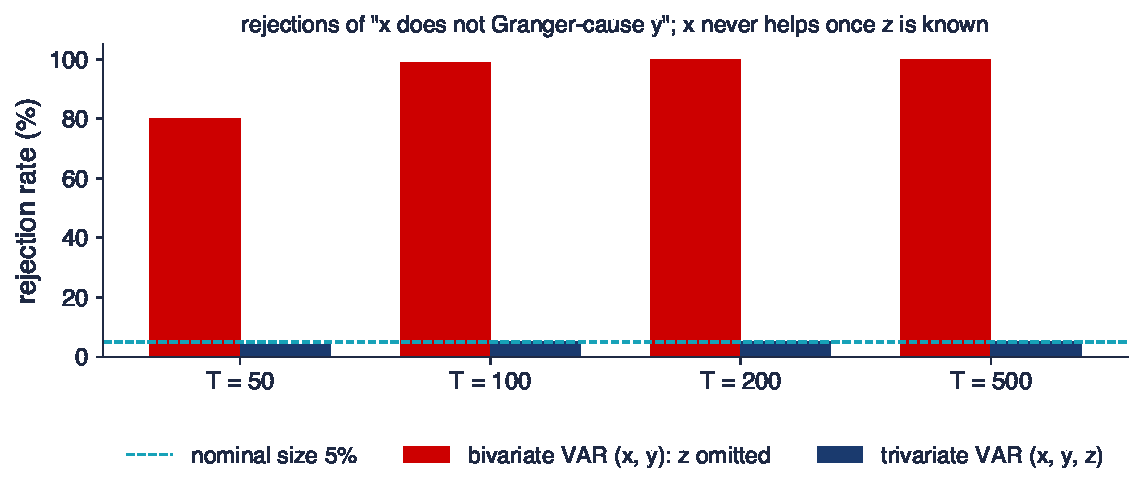
\includegraphics[width=0.97\textwidth,height=0.52\textheight,keepaspectratio]{tsa_ch6_granger_sim.pdf}
\end{center}
\vspace{-0.25cm}
\begin{itemize}
    \item 1\,000 simulations per sample size of the system of the previous slide; $F$ test of ``$x$ does not Granger-cause $y$'' at 5\% in a VAR(2), with and without $z$
\end{itemize}
\quantlet{TSA\_ch6\_granger}{\qlurl{TSA_ch6_granger}}
\end{frame}

\begin{frame}{Interpreting the simulation}
\itemsize{\small}
\begin{itemize}
    \item Without $z$, the test rejects in 80\% of samples with $T = 50$ and 100\% with $T = 200$: almost always a ``cause''
    \begin{itemize}
        \item more data makes it worse: the test becomes more sure of a wrong conclusion
    \end{itemize}
    \item With $z$ in the VAR, the rejection rate is 4.3\%--5.2\%, close to the nominal 5\%
    \begin{itemize}
        \item Granger causality is a property of the chosen system, not of the world
    \end{itemize}
    \item Romanian example: inflation $\to$ GDP growth has p = 0.059 in the three-variable VAR and 0.173 in the bivariate one
\end{itemize}
\end{frame}

\begin{frame}{Pitfall 2: instantaneous causality}
\itemsize{\small}
\begin{itemize}
    \item Granger tests only use lags; effects within the same period are hidden in the correlation of the shocks $\bSigma$
    \begin{itemize}
        \item \textbf{instantaneous causality} between $x$ and $y$: $\Cov(\varepsilon_{xt}, \varepsilon_{yt}) \ne 0$; tested by a Wald test on the off-diagonal elements of $\bSigma$
    \end{itemize}
    \item It has \textbf{no direction}: the data cannot tell whether $x$ moved $y$ or $y$ moved $x$ within the quarter
    \begin{itemize}
        \item Romania: ROBOR shocks are instantaneously correlated with the others (p = 0.041); the residual correlation of inflation and ROBOR is 0.25
    \end{itemize}
    \item With quarterly data, many true effects happen within the quarter: a VAR in which nothing is Granger-significant can still have strong links (Section 7)
\end{itemize}
\end{frame}

\begin{frame}{Pitfall 3: trends, expectations and the meaning of "cause"}
\itemsize{\small}
\begin{itemize}
    \item \textbf{Non-stationary variables}: with $I(1)$ series the $F$ and Wald tests do not have their usual distributions \refSSW
    \begin{itemize}
        \item remedies: test on differences (if there is no cointegration), or the Toda--Yamamoto approach \refTY: estimate a VAR$(p + d_{\max})$ in levels and test only the first $p$ lags
        \item $d_{\max}$: the highest order of integration of the series (usually 1); the extra lags are estimated but not tested
        \item cointegrated series need a VECM: \tsachlink{https://danpele.github.io/Time-Series-Analysis/EN/Courses/chapter7_cointegration_vecm.pdf}{Chapter 7}
    \end{itemize}
    \item \textbf{Expectations}: forward-looking prices move before the events they anticipate
    \begin{itemize}
        \item stock prices Granger-cause GDP, and weather forecasts ``cause'' rain; neither is a cause in the everyday sense
    \end{itemize}
    \item Report: ``$x$ helps to predict $y$, given these variables and this sample''; never ``$x$ causes $y$''
\end{itemize}
\end{frame}

\begin{frame}{Recap: Granger causality}
\itemsize{\small}
\begin{itemize}
    \item $x \to y$ (Granger): the lags of $x$ improve the forecast of $y$; $F$ or Wald test of zero restrictions
    \item Romania: GDP growth and inflation $\to$ ROBOR; markets: S\&P 500 $\to$ DAX, BET (time zones)
    \item Pitfalls: omitted variables, instantaneous effects, non-stationarity, expectations
    \item Granger causality is predictability, not causation
\end{itemize}
\end{frame}


%=============================================================================
\section{Impulse responses}
%=============================================================================

\begin{frame}{Impulse responses and why we orthogonalise}
\itemsize{\small}
\begin{itemize}
    \item \textbf{Impulse response function} (IRF): the path of $Y_{j,t+h}$, $h = 0, 1, 2, \dots$, after a one-time shock to variable $k$ at time $t$
    \begin{itemize}
        \item from the moving-average form: the response to a unit change in $\varepsilon_{kt}$ is the column $k$ of $\bPhi_h$
    \end{itemize}
    \item \textbf{Problem}: the shocks are correlated ($\bSigma$ not diagonal)
    \begin{itemize}
        \item ``a shock to inflation with no shock to ROBOR'' is an experiment that the data rarely show: the two shocks usually come together (correlation 0.25)
    \end{itemize}
    \item \textbf{Solution}: rewrite the shocks as $\bepsilon_t = \mathbf{P}\mathbf{u}_t$, with $\mathbf{u}_t$ uncorrelated, unit variance: $\bSigma = \mathbf{P}\mathbf{P}'$
    \begin{itemize}
        \item the \textbf{orthogonalised} IRF: $\boldsymbol{\Theta}_h = \bPhi_h\mathbf{P}$; element $(j, k)$: the response of $Y_j$ to a one-standard-deviation shock $u_k$
        \item $\mathbf{P}$: a $K \times K$ matrix that turns the uncorrelated shocks $\mathbf{u}_t$ into the observed shocks $\bepsilon_t$
    \end{itemize}
\end{itemize}
\end{frame}

\begin{frame}{The Cholesky decomposition and the ordering}
\itemsize{\small}
\begin{itemize}
    \item \textbf{Cholesky}: the unique lower triangular $\mathbf{P}$ with positive diagonal such that $\bSigma = \mathbf{P}\mathbf{P}'$
    \begin{itemize}
        \item example: $\bSigma = \begin{pmatrix} 1 & 0.5 \\ 0.5 & 1 \end{pmatrix}$: $\mathbf{P} = \begin{pmatrix} 1.000 & 0.000 \\ 0.500 & 0.866 \end{pmatrix}$, since $p_{11} = 1$, $p_{21} = 0.5/1$, $p_{22} = \sqrt{1 - 0.25}$
    \end{itemize}
    \item \textbf{Recursive structure}: $\varepsilon_{1t} = p_{11}u_{1t}$, $\varepsilon_{2t} = p_{21}u_{1t} + p_{22}u_{2t}$
    \begin{itemize}
        \item the first variable is not moved by $u_2$ in the same period; the second reacts to both at once
        \item the whole correlation is attributed to the variable ordered first
    \end{itemize}
    \item \textbf{The ordering matters}: with $y_2$ first, $\mathbf{P} = \begin{pmatrix} 0.866 & 0.500 \\ 0.000 & 1.000 \end{pmatrix}$ (upper triangular in the original order)
    \begin{itemize}
        \item rule: order from the slowest variable (does not react within the period) to the fastest; Romania: GDP growth, inflation, ROBOR
    \end{itemize}
\end{itemize}
\end{frame}

\begin{frame}{Worked example: orthogonalised responses}
\itemsize{\small}
\begin{itemize}
    \item VAR(1) of Section 2, order $(y_1, y_2)$: $\boldsymbol{\Theta}_0 = \mathbf{P} = \begin{pmatrix} 1.000 & 0.000 \\ 0.500 & 0.866 \end{pmatrix}$
    \begin{itemize}
        \item a shock $u_1 = 1$ moves $y_1$ by 1 and $y_2$ by 0.500 at once; $u_2 = 1$ moves only $y_2$, by 0.866
    \end{itemize}
    \item One period later: $\boldsymbol{\Theta}_1 = \bA\mathbf{P} = \begin{pmatrix} 0.600 & 0.173 \\ 0.500 & 0.346 \end{pmatrix}$
    \begin{itemize}
        \item $y_2$ responds to $u_1$ by 0.500: $0.3 \cdot 1 + 0.4 \cdot 0.5$, the direct effect $a_{21}$ plus its own persistence
    \end{itemize}
    \item The \textbf{cumulative} response $\sum_{s \le h}\boldsymbol{\Theta}_s$ gives the effect on the level when the VAR is in growth rates
\end{itemize}
\end{frame}

\begin{frame}{Impulse responses of the Romanian VAR(2)}
\itemsize{\footnotesize}
\begin{center}
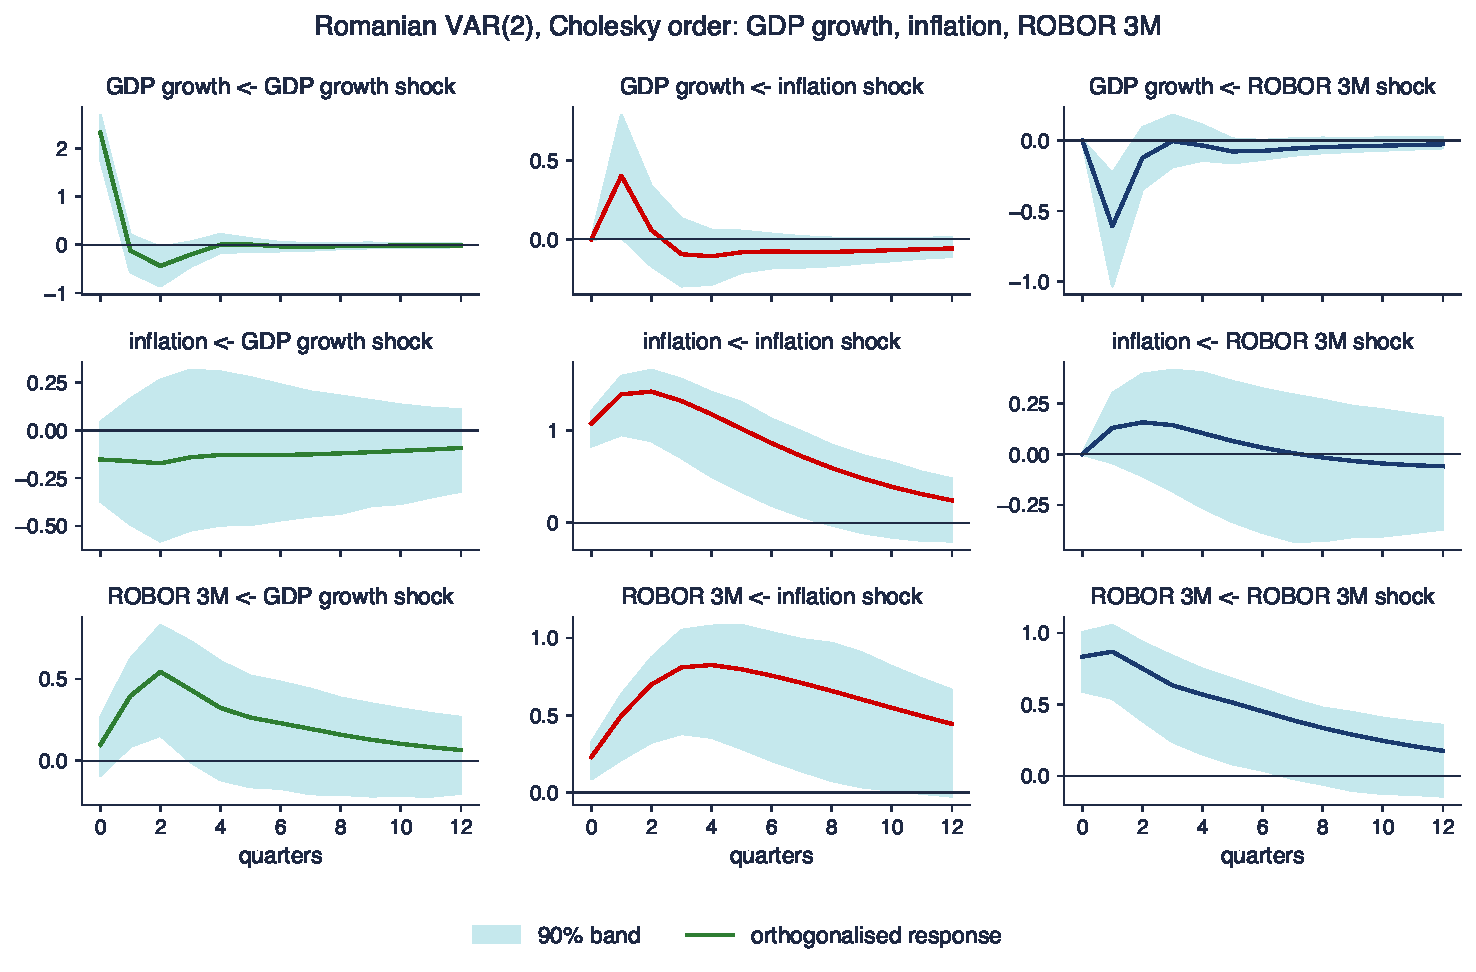
\includegraphics[width=0.97\textwidth,height=0.72\textheight,keepaspectratio]{tsa_ch6_irf_ro.pdf}
\end{center}
\vspace{-0.25cm}
\begin{itemize}
    \item Row: responding variable; column: shock of one standard deviation; Cholesky order $g, \pi, i$; 90\% bands from a residual bootstrap (500 replications) \refKilian
\end{itemize}
\quantlet{TSA\_ch6\_irf\_fevd}{\qlurl{TSA_ch6_irf_fevd}}
\end{frame}

\begin{frame}{Interpreting the Romanian responses}
\itemsize{\small}
\begin{itemize}
    \item An inflation shock (1.08 pp on impact) raises ROBOR by 0.23 pp at once and by up to 0.82 pp after 4 quarters; still 0.44 pp after 3 years
    \begin{itemize}
        \item the band excludes zero for 11 of the 13 horizons: the clearest result of the VAR
    \end{itemize}
    \item A ROBOR shock lowers GDP growth by 0.61 pp the next quarter, then the effect vanishes
    \begin{itemize}
        \item but inflation \textbf{rises} after a ROBOR shock (up to 0.16 pp, not significant): the ``price puzzle'' \refSimsPP
        \item a likely reason: the rate rises when the central bank expects inflation; information omitted from the VAR (exchange rate, energy prices) shows up as a ``shock''
    \end{itemize}
    \item Inflation shocks themselves are persistent: 1.18 pp after a year, 0.24 pp after three
\end{itemize}
\end{frame}

\begin{frame}{Does the ordering change the answer?}
\itemsize{\footnotesize}
\begin{center}
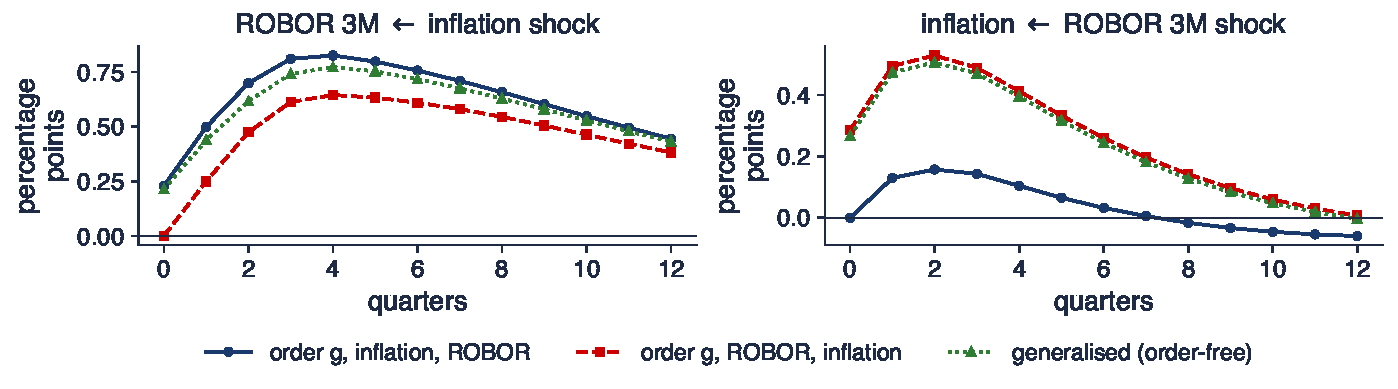
\includegraphics[width=0.97\textwidth,height=0.52\textheight,keepaspectratio]{tsa_ch6_irf_order.pdf}
\end{center}
\vspace{-0.25cm}
\begin{itemize}
    \item Same VAR(2), two Cholesky orderings (inflation before ROBOR, ROBOR before inflation) and the generalised responses of \refPS, which do not depend on the order
\end{itemize}
\quantlet{TSA\_ch6\_irf\_fevd}{\qlurl{TSA_ch6_irf_fevd}}
\end{frame}

\begin{frame}{Interpreting the two orderings}
\itemsize{\small}
\begin{itemize}
    \item ROBOR after an inflation shock: peak 0.82 pp (inflation first) against 0.64 pp (ROBOR first)
    \begin{itemize}
        \item with ROBOR first, the impact response is zero by construction
    \end{itemize}
    \item Inflation after a ROBOR shock: 0.16 pp against 0.53 pp, with 0.29 pp already on impact
    \begin{itemize}
        \item the second ordering assigns the common part of the two shocks (correlation 0.25) to ROBOR, so the ``price puzzle'' gets larger
    \end{itemize}
    \item The ordering is an assumption about which variable reacts within the quarter; it must be stated and defended, and results that change with it are fragile
\end{itemize}
\end{frame}

\begin{frame}{Generalised impulse responses}
\itemsize{\small}
\begin{itemize}
    \item \textbf{Generalised IRF} \refPS\ (after \refKPP): shock variable $k$ by one standard deviation and let the other shocks move as they usually do with it
    \begin{itemize}
        \item $\boldsymbol{\psi}_k(h) = \bPhi_h\bSigma\mathbf{e}_k/\sqrt{\sigma_{kk}}$; $\mathbf{e}_k$: column $k$ of the identity matrix; $\sigma_{kk}$: the variance of shock $k$
    \end{itemize}
    \item Properties
    \begin{itemize}
        \item no ordering is needed; for the variable ordered first, it equals the Cholesky response
        \item the shocks are not orthogonal: the responses to different shocks overlap and cannot be added up
    \end{itemize}
    \item Useful for markets, where no ordering is natural; it describes typical co-movements, not structural shocks
\end{itemize}
\end{frame}

\begin{frame}{Markets: responses to an S\&P 500 shock}
\itemsize{\footnotesize}
\begin{center}
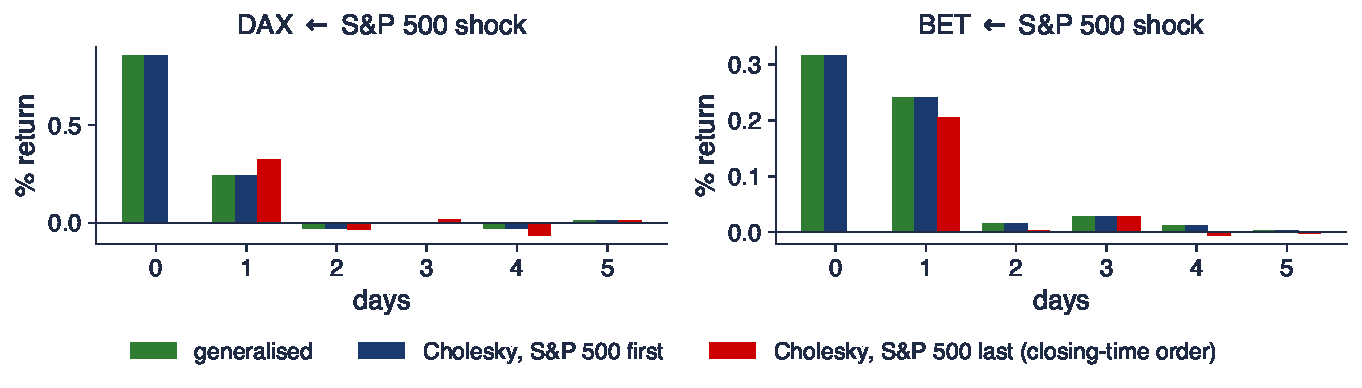
\includegraphics[width=0.97\textwidth,height=0.52\textheight,keepaspectratio]{tsa_ch6_market_irf.pdf}
\end{center}
\vspace{-0.25cm}
\begin{itemize}
    \item VAR(4) of daily S\&P 500, DAX and BET returns; S\&P shock of one standard deviation (1.21\%); generalised responses, Cholesky with the S\&P 500 first, and Cholesky in the order of the closing times (BET, DAX, S\&P 500)
\end{itemize}
\quantlet{TSA\_ch6\_market\_spillovers}{\qlurl{TSA_ch6_market_spillovers}}
\end{frame}

\begin{frame}{Interpreting the market responses}
\itemsize{\small}
\begin{itemize}
    \item Generalised: DAX 0.85\% on the same day and 0.24\% the next; BET 0.32\% and 0.24\%
    \begin{itemize}
        \item identical to the Cholesky responses with the S\&P 500 first, as the theory says
    \end{itemize}
    \item With the S\&P 500 last (it closes last), the same-day response is zero by assumption and the next-day responses are 0.32\% (DAX) and 0.20\% (BET)
    \begin{itemize}
        \item the same-day correlation (0.63 with the DAX) is attributed to Europe in this order
    \end{itemize}
    \item Either way, the effect is over after two days: markets absorb the news quickly
\end{itemize}
\end{frame}

\begin{frame}{Recap: Impulse responses}
\itemsize{\small}
\begin{itemize}
    \item IRF: columns of $\bPhi_h$; orthogonalised: $\boldsymbol{\Theta}_h = \bPhi_h\mathbf{P}$, $\bSigma = \mathbf{P}\mathbf{P}'$
    \item Cholesky = recursive ordering; the ordering is an assumption and can change the results
    \item Romania: ROBOR rises for years after an inflation shock; a ``price puzzle'' appears
    \item Generalised IRF: order-free, but not additive; bootstrap bands for inference
\end{itemize}
\end{frame}


%=============================================================================
\section{Forecast error variance decomposition}
%=============================================================================

\begin{frame}{Forecast error variance decomposition}
\itemsize{\small}
\begin{itemize}
    \item $h$-step forecast error: $\bY_{t+h} - \hat\bY_{t+h|t} = \sum_{s=0}^{h-1}\bPhi_s\bepsilon_{t+h-s} = \sum_{s=0}^{h-1}\boldsymbol{\Theta}_s\mathbf{u}_{t+h-s}$
    \begin{itemize}
        \item the orthogonal shocks $u_k$ are uncorrelated, so the variance splits into $K$ parts
    \end{itemize}
    \item \textbf{FEVD}: $\omega_{jk}(h) = \dfrac{\sum_{s=0}^{h-1}\theta_{jk,s}^2}{\sum_{s=0}^{h-1}\sum_{m=1}^{K}\theta_{jm,s}^2}$, the share of shock $k$ in the $h$-step error variance of $Y_j$
    \begin{itemize}
        \item $\theta_{jk,s}$: element $(j, k)$ of $\boldsymbol{\Theta}_s$; $\hat\bY_{t+h|t}$: the forecast of $\bY_{t+h}$ made at $t$
        \item each row sums to 100\%; it depends on the Cholesky ordering; at $h = 1$ the first variable is explained 100\% by its own shock
    \end{itemize}
    \item Example (VAR(1) of Section 2), $h = 2$: the variance of the error of $y_2$ is 1.37; shock $u_1$ explains 36.5\%
    \begin{itemize}
        \item $(0.5^2 + 0.5^2)/1.37$: the impact $p_{21} = 0.5$ and the next-period response 0.500
    \end{itemize}
\end{itemize}
\end{frame}

\begin{frame}{FEVD of the Romanian VAR(2)}
\itemsize{\footnotesize}
\begin{center}
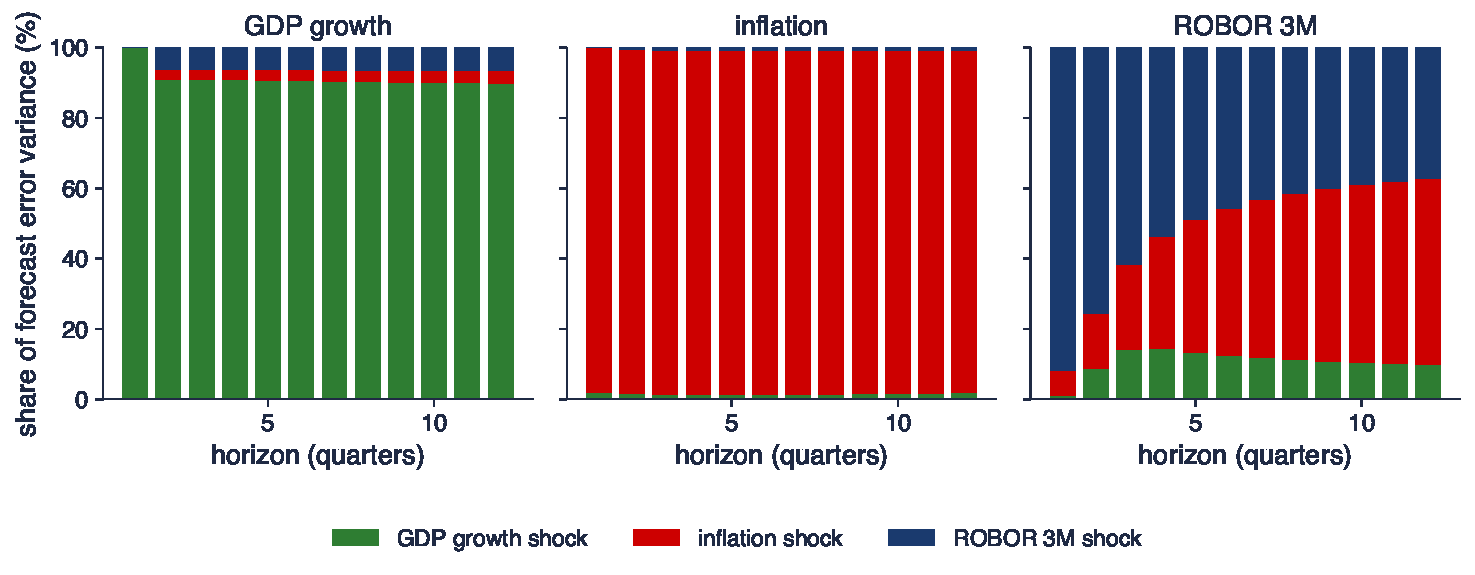
\includegraphics[width=0.97\textwidth,height=0.5\textheight,keepaspectratio]{tsa_ch6_fevd_ro.pdf}
\end{center}
\vspace{-0.25cm}
\begin{itemize}
    \item Share of each orthogonal shock in the forecast error variance, horizons 1--12 quarters, Cholesky order $g, \pi, i$
\end{itemize}
\quantlet{TSA\_ch6\_irf\_fevd}{\qlurl{TSA_ch6_irf_fevd}}
\end{frame}

\begin{frame}{Interpreting the variance decomposition}
\itemsize{\small}
\begin{itemize}
    \item ROBOR: own shocks explain 92\% at one quarter, but only 37\% after three years; inflation shocks explain 53\%, GDP shocks 10\%
    \begin{itemize}
        \item in the long run, the interest rate is mostly driven by inflation
    \end{itemize}
    \item Inflation: 97\% own shocks even after 12 quarters; GDP growth: 90\% own shocks
    \begin{itemize}
        \item in this small VAR, inflation is driven by forces outside the model (energy, food, exchange rate, taxes)
    \end{itemize}
    \item FEVD and Granger tests agree: the information flows from inflation and output to the interest rate
\end{itemize}
\end{frame}

\begin{frame}{Case study: Diebold and Yilmaz (2009, 2012)}
\itemsize{\small}
\begin{itemize}
    \item \textbf{Question}: how much of the forecast uncertainty of one market comes from shocks in other markets, and how does it change over time?
    \begin{itemize}
        \item \refDY: Cholesky FEVD of weekly returns of 19 stock markets; \refDYb: generalised FEVD, which removes the dependence on the ordering
    \end{itemize}
    \item \textbf{Spillover index}: $S(H) = \frac{100}{K}\sum_{j \ne k}\tilde\omega_{jk}(H)$, the average share of other markets' shocks
    \begin{itemize}
        \item $\tilde\omega_{jk}$: generalised FEVD rescaled so that each row sums to 1; the specification of \refDYb: VAR(4), $H = 10$ days, rolling 200-day windows
    \end{itemize}
    \item \textbf{Finding}: spillovers rise sharply in crises; markets become more connected exactly when diversification is most needed
    \begin{itemize}
        \item next: the index for the S\&P 500, the DAX and the BET
    \end{itemize}
\end{itemize}
\end{frame}

\begin{frame}{Spillover table: S\&P 500, DAX, BET}
\itemsize{\small}
\begin{center}
\footnotesize
\begin{tabular}{lrrrr}
\toprule
\textbf{To $\leftarrow$ from (\%)} & S\&P 500 & DAX & BET & \textbf{from others} \\
\midrule
S\&P 500 & 69.2 & 27.1 & 3.7 & 30.8 \\
DAX & 28.2 & 66.4 & 5.4 & 33.6 \\
BET & 7.2 & 7.5 & 85.3 & 14.7 \\
\textbf{to others} & 35.4 & 34.6 & 9.1 & index 26.4 \\
\bottomrule
\end{tabular}
\end{center}
\begin{itemize}
    \item Row $j$: shares of the 10-day forecast error variance of market $j$ due to shocks in each market (generalised FEVD, full sample 2000--2026)
    \item The S\&P 500 receives 27.1\% from the DAX and the DAX 28.2\% from the S\&P 500; the BET receives 14.7\% and gives only 9.1\%: a small, net receiving market
\end{itemize}\quantlet{TSA\_ch6\_market\_spillovers}{\qlurl{TSA_ch6_market_spillovers}}
\end{frame}

\begin{frame}{The spillover index over time}
\itemsize{\footnotesize}
\begin{center}
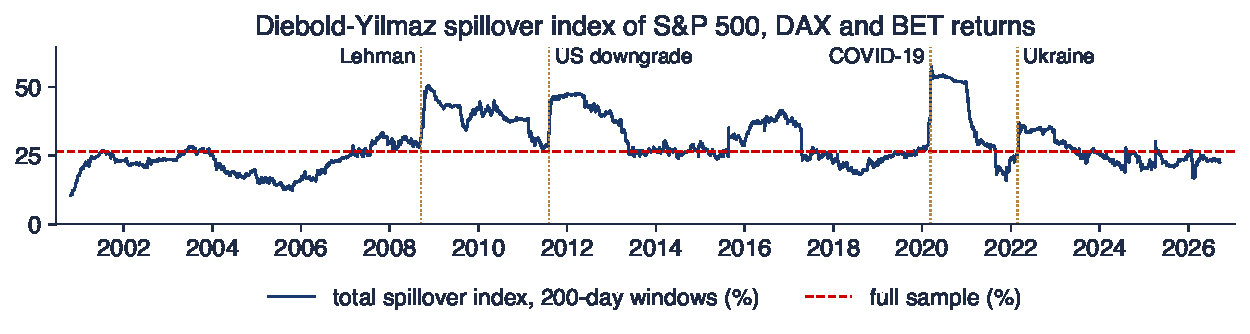
\includegraphics[width=0.97\textwidth,height=0.52\textheight,keepaspectratio]{tsa_ch6_spillover.pdf}
\end{center}
\vspace{-0.25cm}
\begin{itemize}
    \item Total spillover index of S\&P 500, DAX and BET daily returns: generalised FEVD at 10 days from a VAR(4), rolling windows of 200 trading days (29.0\% on average)
\end{itemize}
\quantlet{TSA\_ch6\_market\_spillovers}{\qlurl{TSA_ch6_market_spillovers}}
\end{frame}

\begin{frame}{Interpreting the spillover index}
\itemsize{\small}
\begin{itemize}
    \item From 28\% in 2007 to 47\% in 2008Q4 (after Lehman); maximum 57.5\% on 17 March 2020, in the COVID-19 crash
    \begin{itemize}
        \item the same pattern as in \refDY: connectedness jumps in crises and decays slowly
    \end{itemize}
    \item Most recent value: 22.7\%, below the full-sample index (26.4\%)
    \begin{itemize}
        \item the jumps are partly mechanical: a 200-day window that contains a crash is dominated by it for the next 200 days
    \end{itemize}
    \item For a portfolio holding the BET: diversification across these markets helps least when it is needed most
\end{itemize}
\end{frame}

\begin{frame}{Recap: Variance decomposition}
\itemsize{\small}
\begin{itemize}
    \item FEVD: share of each orthogonal shock in the $h$-step forecast error variance; rows sum to 100\%
    \item Romania: ROBOR is driven by inflation at long horizons; inflation mainly by its own shocks
    \item Diebold--Yilmaz spillover index: the off-diagonal mass of the generalised FEVD
    \item Spillovers among S\&P 500, DAX and BET peak in crises (2008, 2020)
\end{itemize}
\end{frame}


%=============================================================================
\section{Forecasting with a VAR}
%=============================================================================

\begin{frame}{VAR forecasts and their uncertainty}
\itemsize{\small}
\begin{itemize}
    \item \textbf{Point forecasts} by recursion: $\hat\bY_{T+h|T} = \bc + \bA_1\hat\bY_{T+h-1|T} + \dots + \bA_p\hat\bY_{T+h-p|T}$, with $\hat\bY_{T+j|T} = \bY_{T+j}$ for $j \le 0$
    \begin{itemize}
        \item for a stable VAR they converge to the mean $\boldsymbol{\mu}$ as $h$ grows
    \end{itemize}
    \item \textbf{Error covariance}: $\bSigma(h) = \sum_{s=0}^{h-1}\bPhi_s\bSigma\bPhi_s'$; it grows with $h$ towards $\bGamma(0)$
    \begin{itemize}
        \item 95\% interval for $Y_j$: $\hat Y_{j,T+h|T} \pm 1.96\sqrt{\sigma_{jj}(h)}$, $\sigma_{jj}(h)$: element $(j, j)$ of $\bSigma(h)$ (Normal shocks; parameter uncertainty ignored)
        \item example (Section 2): $\bSigma(2) = \bSigma + \bA\bSigma\bA'$, with variances 1.39 and 1.37
    \end{itemize}
    \item Same logic as the ARMA forecasts of \tsachlink{https://danpele.github.io/Time-Series-Analysis/EN/Courses/chapter2_arma_models.pdf}{Chapter 2}, with matrices in place of numbers
\end{itemize}
\end{frame}

\begin{frame}{Romanian VAR(2): forecasts for two years}
\itemsize{\footnotesize}
\begin{center}
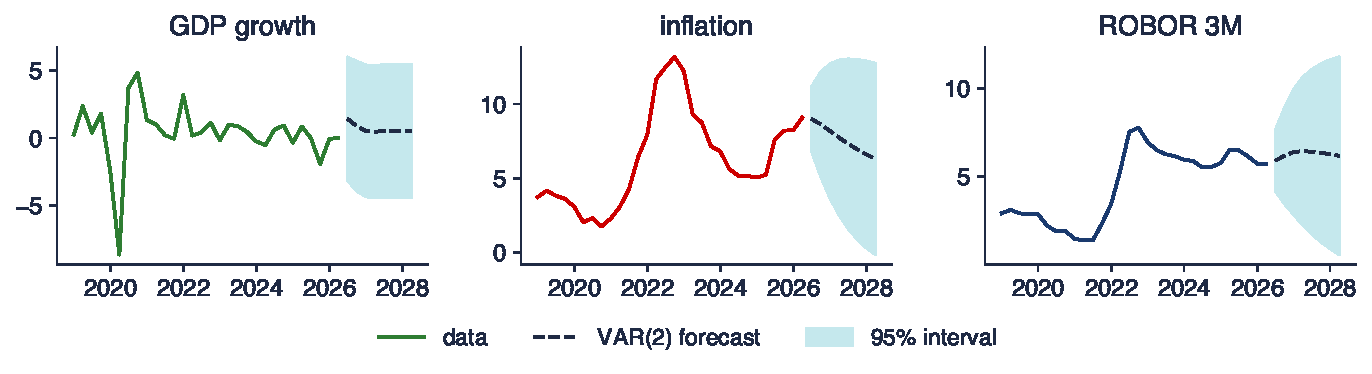
\includegraphics[width=0.97\textwidth,height=0.5\textheight,keepaspectratio]{tsa_ch6_forecast_ro.pdf}
\end{center}
\vspace{-0.25cm}
\begin{itemize}
    \item Data until 2026Q2; forecasts 2026Q3--2028Q2 with 95\% intervals
\end{itemize}
\quantlet{TSA\_ch6\_forecasting}{\qlurl{TSA_ch6_forecasting}}
\end{frame}

\begin{frame}{Interpreting the forecasts}
\itemsize{\small}
\begin{itemize}
    \item Inflation: from 9.1\% in 2026Q2 to 7.7\% after a year and 6.3\% after two (95\%: $[-0.1, 12.7]$)
    \begin{itemize}
        \item the forecasts move towards the VAR mean (inflation 4.8\%, ROBOR 4.8\%), slowly because the largest eigenvalue is 0.869
    \end{itemize}
    \item ROBOR: 6.4\% after a year, 6.2\% after two; GDP growth: 0.5\% per quarter, with an interval $[-4.4, 5.3]$
    \begin{itemize}
        \item the GDP interval is wide because the 2009 and 2020 outliers inflate $\hat\sigma_g$
    \end{itemize}
    \item A mechanical forecast: it knows nothing of the budget, energy prices or BNR decisions; its value is as a transparent benchmark
\end{itemize}
\end{frame}

\begin{frame}{Evaluating VAR forecasts fairly}
\itemsize{\small}
\begin{itemize}
    \item \textbf{Pseudo out-of-sample}: re-estimate on data up to $t$ only, forecast $t + h$, move $t$ forward (expanding window)
    \begin{itemize}
        \item never evaluate on the data used for estimation (\tsachlink{https://danpele.github.io/Time-Series-Analysis/EN/Courses/chapter0_introduction.pdf}{Chapter 0})
    \end{itemize}
    \item \textbf{Benchmarks}: the random walk (no change) and a univariate AR$(p)$ for each variable, $p$ by AIC
    \begin{itemize}
        \item the question is not ``is the VAR good?'', but ``do the other variables add anything to the series' own past?''
    \end{itemize}
    \item Measures: RMSE relative to the random walk (below 1: better); the Diebold--Mariano test \refDM\ for equal accuracy
    \begin{itemize}
        \item DM statistic: the mean difference of squared errors divided by its standard error; approximately $N(0, 1)$ under $H_0$
    \end{itemize}
\end{itemize}
\end{frame}

\begin{frame}{VAR against univariate benchmarks}
\itemsize{\footnotesize}
\begin{center}
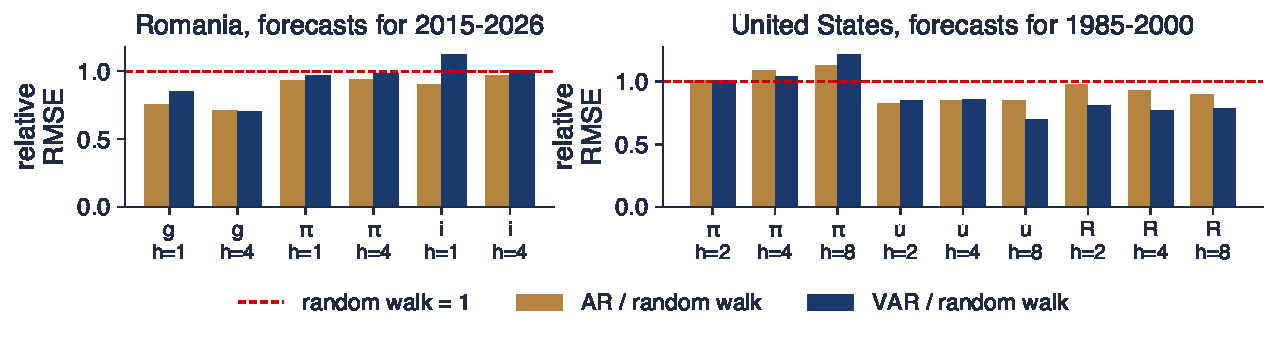
\includegraphics[width=0.97\textwidth,height=0.5\textheight,keepaspectratio]{tsa_ch6_oos.pdf}
\end{center}
\vspace{-0.25cm}
\begin{itemize}
    \item Relative RMSE (model / random walk). Left: Romania, 46 forecasts per horizon, origins 2014Q4--2026Q1; right: the US VAR of Section 10, forecasts for 1985Q1--2000Q4, the evaluation period of \refSW
\end{itemize}
\quantlet{TSA\_ch6\_forecasting}{\qlurl{TSA_ch6_forecasting}}
\end{frame}

\begin{frame}{Interpreting the forecast comparison}
\itemsize{\small}
\begin{itemize}
    \item Romania, one quarter ahead: the VAR loses to the AR for GDP growth (0.85 against 0.75; DM = 2.59, p = 0.010) and is no better for inflation or ROBOR
    \begin{itemize}
        \item 21 coefficients on 38 to 84 quarters: the estimation noise eats the information of the other variables
    \end{itemize}
    \item United States, 8 quarters ahead: the VAR beats the AR for unemployment (0.70 against 0.85) and the fed funds rate (0.79 against 0.90)
    \begin{itemize}
        \item for inflation, nothing beats the random walk (1.22) at this horizon in this period
    \end{itemize}
    \item VARs help when the sample is long and the links are strong; in short, noisy samples a simple AR is hard to beat
\end{itemize}
\end{frame}

\begin{frame}{Recap: Forecasting with a VAR}
\itemsize{\small}
\begin{itemize}
    \item Recursive point forecasts; error covariance $\sum_s\bPhi_s\bSigma\bPhi_s'$
    \item Evaluate out of sample against the random walk and univariate AR models
    \item Romania: no gain from the VAR; US 1985--2000: gains for unemployment and the interest rate
\end{itemize}
\end{frame}


%=============================================================================
\section{Structural VARs and a landmark case study}
%=============================================================================

\begin{frame}{From reduced form to structural VAR}
\itemsize{\small}
\begin{itemize}
    \item \textbf{Structural VAR} (SVAR): $\mathbf{B}_0\bY_t = \mathbf{d} + \mathbf{B}_1\bY_{t-1} + \dots + \mathbf{B}_p\bY_{t-p} + \mathbf{u}_t$, $\mathbf{u}_t$ uncorrelated \textbf{structural shocks}
    \begin{itemize}
        \item $\mathbf{d}$: constants; $\mathbf{B}_1, \dots, \mathbf{B}_p$: structural lag coefficients; $\mathbf{B}_0$: the contemporaneous effects (e.g.\ the policy rate reacts to this quarter's inflation)
        \item multiplying by $\mathbf{B}_0^{-1}$ gives the reduced form, with $\bepsilon_t = \mathbf{B}_0^{-1}\mathbf{u}_t$
    \end{itemize}
    \item \textbf{Identification}: $\bSigma$ has $K(K+1)/2$ distinct elements, $\mathbf{B}_0^{-1}$ has $K^2$; we need $K(K-1)/2$ restrictions
    \begin{itemize}
        \item Cholesky: $\mathbf{B}_0^{-1} = \mathbf{P}$ lower triangular: exactly $K(K-1)/2$ zeros; the recursive SVAR of \refSims
        \item other schemes: long-run restrictions, sign restrictions, external instruments (beyond this course)
    \end{itemize}
    \item The data identify the reduced form; the structural interpretation always rests on assumptions that must be argued with economics
\end{itemize}
\end{frame}

\begin{frame}{Case study: Stock and Watson (2001)}
\itemsize{\footnotesize}
\begin{columns}[T]
\begin{column}{0.4\textwidth}
\centering

\includegraphics[height=0.3\textheight]{ch6_eccles_building_2011.jpg}\\[1mm]
\imgcap{Eccles Building, Washington: the Federal Reserve Board}
\imgcredit{https://commons.wikimedia.org/wiki/File:Eccles_Building_(26088200676).jpg}{Photo: Federal Reserve (2011); public domain; Wikimedia Commons}
\end{column}
\begin{column}{0.58\textwidth}
\begin{itemize}
    \item \refSW: ``Vector autoregressions'', a widely used survey of the method
    \begin{itemize}
        \item three variables: inflation $\pi_t$, unemployment $u_t$, the federal funds rate $R_t$
        \item $\pi_t = 400\ln(P_t/P_{t-1})$, $P_t$: the GDP price index; 400 annualises, in \%
        \item quarterly, 1960Q1--2000Q4, VAR(4), Cholesky order $\pi, u, R$
    \end{itemize}
    \item Four tasks: data description, forecasting, structural inference, policy analysis
    \begin{itemize}
        \item their verdict: VARs are good at the first two; the last two depend on the identifying assumptions
    \end{itemize}
    \item We re-estimate it with today's FRED data (series GDPCTPI, UNRATE, FEDFUNDS): the numbers differ slightly from the published ones because the data have been revised
\end{itemize}
\end{column}
\end{columns}
\end{frame}

\begin{frame}{The three US series}
\itemsize{\footnotesize}
\begin{center}
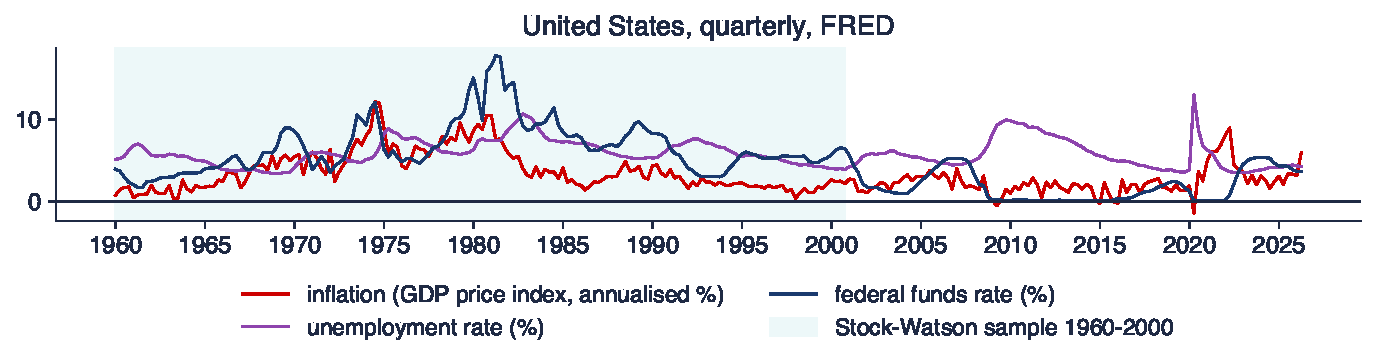
\includegraphics[width=0.97\textwidth,height=0.52\textheight,keepaspectratio]{tsa_ch6_us_data.pdf}
\end{center}
\vspace{-0.25cm}
\begin{itemize}
    \item Quarterly, 1960Q1--2026Q2 (FRED); shaded: the sample of \refSW, 164 quarters
\end{itemize}
\quantlet{TSA\_ch6\_stock\_watson}{\qlurl{TSA_ch6_stock_watson}}
\end{frame}

\begin{frame}{Stock--Watson VAR: impulse responses}
\itemsize{\footnotesize}
\begin{center}
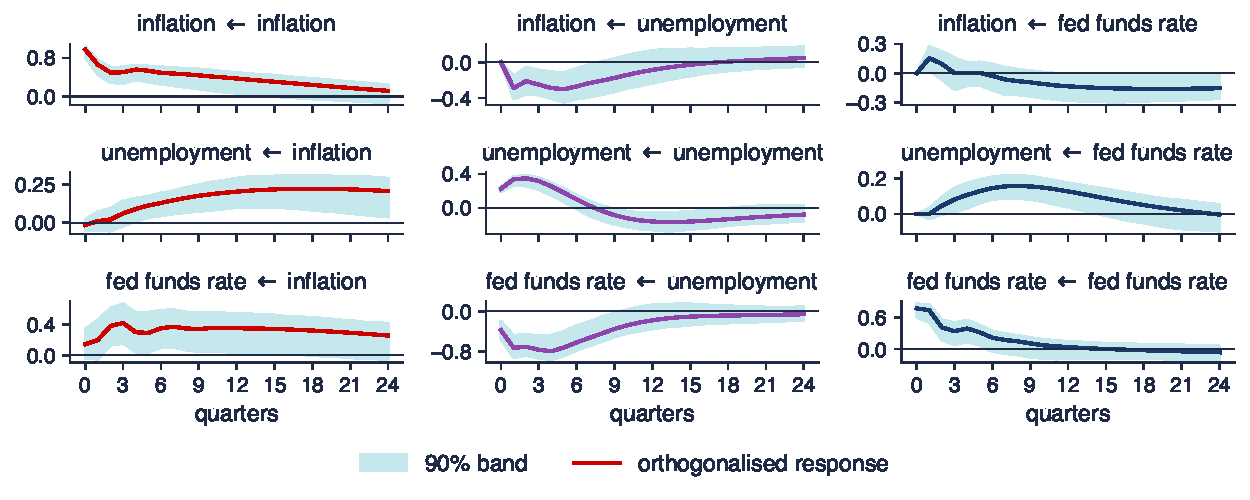
\includegraphics[width=0.97\textwidth,height=0.72\textheight,keepaspectratio]{tsa_ch6_sw_irf.pdf}
\end{center}
\vspace{-0.25cm}
\begin{itemize}
    \item VAR(4), 1960Q1--2000Q4, 39 coefficients; Cholesky order inflation, unemployment, fed funds rate; 24 quarters; 90\% bootstrap bands
\end{itemize}
\quantlet{TSA\_ch6\_stock\_watson}{\qlurl{TSA_ch6_stock_watson}}
\end{frame}

\begin{frame}{Interpreting the Stock--Watson VAR}
\itemsize{\small}
\begin{itemize}
    \item A monetary shock ($+0.78$ pp in the fed funds rate) raises unemployment by up to 0.16 pp after 8 quarters
    \begin{itemize}
        \item inflation first rises (0.16 pp, a price puzzle), then falls slowly ($-$0.13 pp after 3 years)
    \end{itemize}
    \item Granger tests: unemployment $\to$ inflation (p = 0.036), inflation and unemployment $\to$ fed funds (p $<$\,0.001, $<$\,0.001), fed funds $\to$ inflation not significant (p = 0.402)
    \begin{itemize}
        \item FEVD after 12 quarters: monetary shocks explain 19\% of unemployment and 2\% of inflation
    \end{itemize}
    \item On the extended sample 1960--2026Q2 ($T = 262$) the unemployment response has the wrong sign in the first quarters ($-$0.13 pp): zero rates after 2008 and the pandemic change the system
\end{itemize}
\end{frame}

\begin{frame}{The legacy of the VAR}
\itemsize{\small}
\begin{columns}[T]
\begin{column}{0.5\textwidth}
\centering
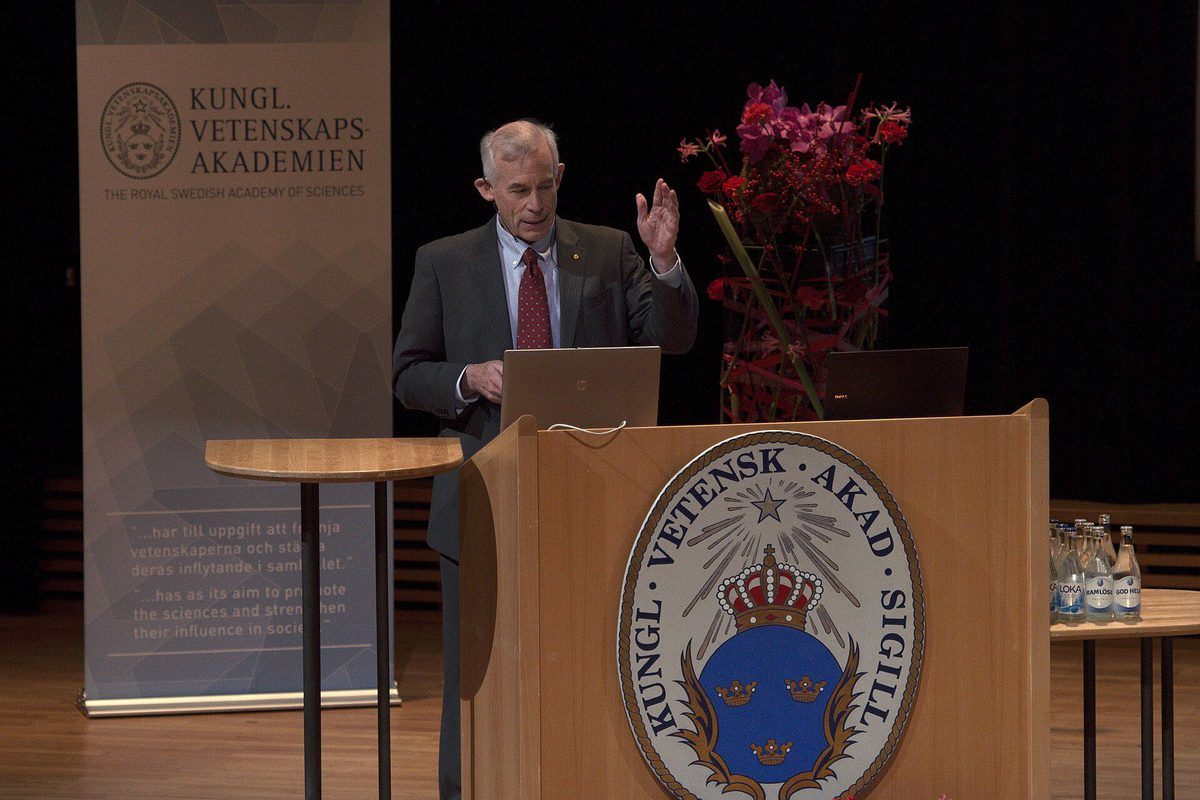
\includegraphics[height=0.4\textheight]{ch6_sims_nobel_lecture_2011.jpg}\\[1mm]
\imgcap{Christopher Sims giving his Nobel lecture, Stockholm, 8 December 2011}
\imgcredit{https://commons.wikimedia.org/wiki/File:Nobel_Prize_2011-Nobel_lectures_KVA-DSC_8085.jpg}{Photo: Holger Motzkau (2011); CC BY-SA 3.0; Wikimedia Commons}
\end{column}
\begin{column}{0.48\textwidth}
\begin{itemize}
    \item Central banks use VARs for forecasts and policy scenarios
    \begin{itemize}
        \item and their descendants: Bayesian VARs, DSGE models compared with VARs
    \end{itemize}
    \item The price puzzle \refSimsPP
    \begin{itemize}
        \item led to adding commodity prices and expectations to monetary VARs
    \end{itemize}
    \item Non-stationary variables that move together need the error-correction form
    \begin{itemize}
        \item \tsachlink{https://danpele.github.io/Time-Series-Analysis/EN/Courses/chapter7_cointegration_vecm.pdf}{Chapter 7}: cointegration and VECM \refEG
    \end{itemize}
\end{itemize}
\end{column}
\end{columns}
\end{frame}

\begin{frame}{Recap: Structural VARs}
\itemsize{\small}
\begin{itemize}
    \item SVAR: $\bepsilon_t = \mathbf{B}_0^{-1}\mathbf{u}_t$; $K(K-1)/2$ restrictions identify the structural shocks
    \item Cholesky is the simplest (recursive) identification
    \item Stock and Watson (2001): a monetary shock raises unemployment; inflation reacts slowly
    \item Results depend on the sample and on the identification
\end{itemize}
\end{frame}


%=============================================================================
\section{Possible contribution of AI}
%=============================================================================

\begin{frame}{Possible contribution of AI}
\itemsize{\small}
\begin{itemize}
    \item \textbf{Code}: a first draft of a script that downloads several series, aligns their dates, selects $p$ and estimates a VAR
    \item \textbf{Explanation}: a second explanation of the Cholesky decomposition or of a FEVD table
    \item \textbf{Exploration}: Granger tests and spillover indices for many pairs of markets or EU countries at once
    \item Example prompt
    \begin{itemize}
        \item \aiprompt{Write Python code that builds a quarterly data set for Romania (real GDP growth from Eurostat namq\_10\_gdp, 12-month HICP inflation from prc\_hicp\_minr, ROBOR 3M from irt\_st\_m), chooses the VAR lag order by AIC, BIC and HQ, checks stability and residuals, runs Granger tests and plots orthogonalised impulse responses with bootstrap bands.}
    \end{itemize}
\end{itemize}
\end{frame}

\begin{frame}{Checks you must run}
\itemsize{\small}
\begin{itemize}
    \item The dates: series aligned on the same quarters, no forward-filled or overlapping values that create spurious leads
    \item Stationarity of each variable (\tsachlink{https://danpele.github.io/Time-Series-Analysis/EN/Courses/chapter3_unit_roots_arima_models.pdf}{Chapter 3}) before Granger tests; with $I(1)$ variables, differences, Toda--Yamamoto or a VECM
    \item Stability from the companion matrix, not from $\bA_1$ alone
    \item The Cholesky ordering used and its justification; the same results with another ordering or with generalised responses
    \item That ``Granger-causes'' is never reported as ``causes''
    \item Every cited reference: it must exist; check the DOI
\end{itemize}
\end{frame}


%=============================================================================
\section{Summary}
%=============================================================================

\begin{frame}{Key takeaways}
\itemsize{\small}
\begin{itemize}
    \item A VAR$(p)$ regresses each variable on the past of all; OLS equation by equation; few variables and lags
    \item Stability: all eigenvalues of the companion matrix inside the unit circle; then a mean and a moving-average form exist
    \item Choose $p$ with AIC, BIC, HQ, then check the residuals with the portmanteau test
    \item Granger causality = incremental predictability, relative to the chosen variables
    \item IRF and FEVD need orthogonal shocks: the Cholesky ordering is an identifying assumption
    \item VAR forecasts must beat AR and random-walk benchmarks out of sample; often they do not
\end{itemize}
\end{frame}

\begin{frame}{Key formulas}
\itemsize{\small}
{\renewcommand{\arraystretch}{1.35}\begin{center}
\footnotesize
\begin{tabular}{ll}
\toprule
\textbf{Quantity} & \textbf{Formula} \\
\midrule
VAR$(p)$ & $\bY_t = \bc + \bA_1\bY_{t-1} + \dots + \bA_p\bY_{t-p} + \bepsilon_t$, \quad $E[\bepsilon_t\bepsilon_t'] = \bSigma$ \\
Stability, mean & $|\lambda_i(\mathbf{F})| < 1$; \quad $\boldsymbol{\mu} = (\mathbf{I} - \bA_1 - \dots - \bA_p)^{-1}\bc$ \\
Criteria & $\ln\det\tilde\bSigma(p) + c_T\,pK^2/T$, \quad $c_T = 2,\ \ln T,\ 2\ln\ln T$ \\
Portmanteau & $Q_h \sim \chi^2(K^2(h - p))$ \\
Granger $F$ & $\dfrac{(RSS_R - RSS_U)/p}{RSS_U/(T - Kp - 1)} \sim F(p, T - Kp - 1)$ \\
MA form, IRF & $\bPhi_h = \sum_{j=1}^{\min(h,p)}\bA_j\bPhi_{h-j}$, \quad $\boldsymbol{\Theta}_h = \bPhi_h\mathbf{P}$, \quad $\bSigma = \mathbf{P}\mathbf{P}'$ \\
FEVD & $\omega_{jk}(h) = \sum_{s<h}\theta_{jk,s}^2 / \sum_{s<h}\sum_m\theta_{jm,s}^2$ \\
Forecast error & $\bSigma(h) = \sum_{s=0}^{h-1}\bPhi_s\bSigma\bPhi_s'$ \\
\bottomrule
\end{tabular}
\end{center}
}
\end{frame}

\begin{frame}{Self-assessment}
\itemsize{\small}
\begin{itemize}
    \item \textbf{Question}: is the VAR(1) with $\bA = \begin{pmatrix} 0.9 & 0.3 \\ 0.2 & 0.8 \end{pmatrix}$ stable?
    \begin{itemize}
        \item \textbf{Answer}: no: $\lambda^2 - 1.7\lambda + 0.66 = 0$ gives $\lambda = 1.1$ and $0.6$
    \end{itemize}
    \item \textbf{Question}: a Granger test gives p = 0.30 for $x \to y$. Does $x$ have no effect on $y$?
    \begin{itemize}
        \item \textbf{Answer}: no such conclusion: the lags of $x$ do not improve the forecast; effects within the period, slow effects or low power remain possible
    \end{itemize}
    \item \textbf{Question}: in a Cholesky FEVD, what share of the 1-step error variance of the first variable comes from its own shock?
    \begin{itemize}
        \item \textbf{Answer}: 100\%, by construction of the ordering
    \end{itemize}
    \item Next: \tsachlink{https://danpele.github.io/Time-Series-Analysis/EN/Courses/chapter7_cointegration_vecm.pdf}{Chapter 7}, cointegration and the vector error correction model (VECM)
\end{itemize}
\end{frame}


%=============================================================================
\section{References}
%=============================================================================

\begin{frame}{References (1/3)}
\itemsize{\scriptsize}
\begin{itemize}
    \item Akaike, H. (1974). A new look at the statistical model identification. \textit{IEEE Transactions on Automatic Control}, 19(6), 716--723. \href{https://doi.org/10.1109/TAC.1974.1100705}{doi:10.1109/TAC.1974.1100705}
    \item Diebold, F. X., \& Mariano, R. S. (1995). Comparing predictive accuracy. \textit{Journal of Business \& Economic Statistics}, 13(3), 253--263. \href{https://doi.org/10.1080/07350015.1995.10524599}{doi:10.1080/07350015.1995.10524599}
    \item Diebold, F. X., \& Yilmaz, K. (2009). Measuring financial asset return and volatility spillovers, with application to global equity markets. \textit{The Economic Journal}, 119(534), 158--171. \href{https://doi.org/10.1111/j.1468-0297.2008.02208.x}{doi:10.1111/j.1468-0297.2008.02208.x}
    \item Diebold, F. X., \& Yilmaz, K. (2012). Better to give than to receive: Predictive directional measurement of volatility spillovers. \textit{International Journal of Forecasting}, 28(1), 57--66. \href{https://doi.org/10.1016/j.ijforecast.2011.02.006}{doi:10.1016/j.ijforecast.2011.02.006}
    \item Engle, R. F., \& Granger, C. W. J. (1987). Co-integration and error correction: Representation, estimation, and testing. \textit{Econometrica}, 55(2), 251--276. \href{https://doi.org/10.2307/1913236}{doi:10.2307/1913236}
    \item Granger, C. W. J. (1969). Investigating causal relations by econometric models and cross-spectral methods. \textit{Econometrica}, 37(3), 424--438. \href{https://doi.org/10.2307/1912791}{doi:10.2307/1912791}
    \item Hamilton, J. D. (1994). \textit{Time Series Analysis}. Princeton University Press. \href{https://doi.org/10.2307/j.ctv14jx6sm}{doi:10.2307/j.ctv14jx6sm}
    \item Hannan, E. J., \& Quinn, B. G. (1979). The determination of the order of an autoregression. \textit{Journal of the Royal Statistical Society: Series B}, 41(2), 190--195. \href{https://doi.org/10.1111/j.2517-6161.1979.tb01072.x}{doi:10.1111/j.2517-6161.1979.tb01072.x}
\end{itemize}
\end{frame}

\begin{frame}{References (2/3)}
\itemsize{\scriptsize}
\begin{itemize}
    \item Hosking, J. R. M. (1980). The multivariate portmanteau statistic. \textit{Journal of the American Statistical Association}, 75(371), 602--608. \href{https://doi.org/10.1080/01621459.1980.10477520}{doi:10.1080/01621459.1980.10477520}
    \item Huang, C., \& Petukhina, A. (2022). \textit{Applied Time Series Analysis and Forecasting with Python}. Springer. \href{https://doi.org/10.1007/978-3-031-13584-2}{doi:10.1007/978-3-031-13584-2}
    \item Hyndman, R. J., \& Athanasopoulos, G. (2021). \textit{Forecasting: Principles and Practice} (3rd ed.), Section 12.3, Vector autoregressions. OTexts. \href{https://otexts.com/fpp3/VAR.html}{otexts.com/fpp3/VAR.html}
    \item Jarque, C. M., \& Bera, A. K. (1980). Efficient tests for normality, homoscedasticity and serial independence of regression residuals. \textit{Economics Letters}, 6(3), 255--259. \href{https://doi.org/10.1016/0165-1765(80)90024-5}{doi:10.1016/0165-1765(80)90024-5}
    \item Kilian, L. (1998). Small-sample confidence intervals for impulse response functions. \textit{Review of Economics and Statistics}, 80(2), 218--230. \href{https://doi.org/10.1162/003465398557465}{doi:10.1162/003465398557465}
    \item Koop, G., Pesaran, M. H., \& Potter, S. M. (1996). Impulse response analysis in nonlinear multivariate models. \textit{Journal of Econometrics}, 74(1), 119--147. \href{https://doi.org/10.1016/0304-4076(95)01753-4}{doi:10.1016/0304-4076(95)01753-4}
    \item Lütkepohl, H. (1982). Non-causality due to omitted variables. \textit{Journal of Econometrics}, 19(2--3), 367--378. \href{https://doi.org/10.1016/0304-4076(82)90011-2}{doi:10.1016/0304-4076(82)90011-2}
\end{itemize}
\end{frame}

\begin{frame}{References (3/3)}
\itemsize{\scriptsize}
\begin{itemize}
    \item Lütkepohl, H. (2005). \textit{New Introduction to Multiple Time Series Analysis}. Springer. \href{https://doi.org/10.1007/978-3-540-27752-1}{doi:10.1007/978-3-540-27752-1}
    \item Pesaran, M. H., \& Shin, Y. (1998). Generalized impulse response analysis in linear multivariate models. \textit{Economics Letters}, 58(1), 17--29. \href{https://doi.org/10.1016/S0165-1765(97)00214-0}{doi:10.1016/S0165-1765(97)00214-0}
    \item Schwarz, G. (1978). Estimating the dimension of a model. \textit{The Annals of Statistics}, 6(2), 461--464. \href{https://doi.org/10.1214/aos/1176344136}{doi:10.1214/aos/1176344136}
    \item Sims, C. A. (1980). Macroeconomics and reality. \textit{Econometrica}, 48(1), 1--48. \href{https://doi.org/10.2307/1912017}{doi:10.2307/1912017}
    \item Sims, C. A. (1992). Interpreting the macroeconomic time series facts: The effects of monetary policy. \textit{European Economic Review}, 36(5), 975--1000. \href{https://doi.org/10.1016/0014-2921(92)90041-T}{doi:10.1016/0014-2921(92)90041-T}
    \item Sims, C. A., Stock, J. H., \& Watson, M. W. (1990). Inference in linear time series models with some unit roots. \textit{Econometrica}, 58(1), 113--144. \href{https://doi.org/10.2307/2938337}{doi:10.2307/2938337}
    \item Stock, J. H., \& Watson, M. W. (2001). Vector autoregressions. \textit{Journal of Economic Perspectives}, 15(4), 101--115. \href{https://doi.org/10.1257/jep.15.4.101}{doi:10.1257/jep.15.4.101}
    \item Toda, H. Y., \& Yamamoto, T. (1995). Statistical inference in vector autoregressions with possibly integrated processes. \textit{Journal of Econometrics}, 66(1--2), 225--250. \href{https://doi.org/10.1016/0304-4076(94)01616-8}{doi:10.1016/0304-4076(94)01616-8}
\end{itemize}
\end{frame}

\end{document}
